\documentclass{article}
\usepackage{amsfonts}
\usepackage{amsmath}
\usepackage{amssymb}
\usepackage{centernot}
\usepackage{hyperref}
\usepackage[none]{hyphenat}
\usepackage{mathrsfs}
\usepackage{mathtools}
\usepackage{physics}
\usepackage{tikz-cd}
\usepackage{tikz}



\parindent=0pt
\usetikzlibrary{positioning}



\title{\textbf{Notes on the book: \\
\emph{Atiyah and Macdonald, Introduction to Commutative Algebra}}}
\author{Meng-Gen Tsai \\ plover@gmail.com}



\begin{document}
\maketitle
\tableofcontents



%%%%%%%%%%%%%%%%%%%%%%%%%%%%%%%%%%%%%%%%%%%%%%%%%%%%%%%%%%%%%%%%%%%%%%%%%%%%%%%%
%%%%%%%%%%%%%%%%%%%%%%%%%%%%%%%%%%%%%%%%%%%%%%%%%%%%%%%%%%%%%%%%%%%%%%%%%%%%%%%%



% Reference:
% https://spaces.ac.cn/usr/uploads/2017/07/4208763092.pdf
% https://www.math.arizona.edu/~cais/371Page/homework/371s1.pdf
% https://math.mit.edu/~jhirsh/notes2_zariski.pdf
% http://yyao.gsucreate.org/math831/831-2.pdf
% http://www.math.ncku.edu.tw/~fjmliou/alg/base.pdf
% https://ocw.mit.edu/courses/mathematics/18-726-algebraic-geometry-spring-2009/lecture-notes/MIT18_726s09_lec11_more_schemes.pdf
% https://www.math.arizona.edu/~jtaylor/notes/atiyah_macdonald_solutions.pdf



%%%%%%%%%%%%%%%%%%%%%%%%%%%%%%%%%%%%%%%%%%%%%%%%%%%%%%%%%%%%%%%%%%%%%%%%%%%%%%%%
%%%%%%%%%%%%%%%%%%%%%%%%%%%%%%%%%%%%%%%%%%%%%%%%%%%%%%%%%%%%%%%%%%%%%%%%%%%%%%%%



\newpage
\section*{Chapter 1: Rings and Ideals \\}
\addcontentsline{toc}{section}{Chapter 1: Rings and Ideals}



\subsubsection*{Exercise 1.1.}
\addcontentsline{toc}{subsubsection}{Exercise 1.1.}
\emph{Let $x$ be a nilpotent element of $A$.
Show that $1+x$ is a unit of $A$.
Deduce that the sum of a nilpotent element and a unit is a unit.} \\



\emph{Proof.}
\begin{enumerate}
\item[(1)]
  Suppose $x^m = 0$ for some odd integer $m \geq 0$.
  Then
  \[
    1 = 1+x^m = (1+x)(1-x+x^2-\cdots+(-1)^{m-1}x^{m-1}),
  \]
  or $1+x$ is a unit.

\item[(2)]
  If $u$ is any unit and $x$ is any nilpotent,
  $u + x= u \cdot (1 + u^{-1}x)$ is a product of two units
  (using that $u^{-1}x$ is nilpotent and applying (1))
  and hence a unit again.
\end{enumerate}
$\Box$ \\



\emph{Proof (Proposition 1.9).}
\begin{enumerate}
\item[(1)]
  \emph{The nilradical is a subset of the Jacobson radical.}
  \begin{enumerate}
  \item[(a)]
    The nilradical $\mathfrak{N}$ of $A$ is the intersection of all the prime ideals of $A$
    by Proposition 1.8.
  \item[(b)]
    The Jacobson radical $\mathfrak{J}$ of $A$ is
    the intersection of all the maximal ideals of $A$
    by definition.
  \end{enumerate}

\item[(2)]
  By Proposition 1.9,
  $x \in \mathfrak{J}$ if and only if
  $1-xy$ is a unit in $A$ for all $y \in A$.
  So $1+x = 1 - (-x) \cdot 1$ is a unit in $A$
  since $x$ is a nilpotent and $\mathfrak{J}$ is an ideal.
\end{enumerate}
$\Box$ \\\\



%%%%%%%%%%%%%%%%%%%%%%%%%%%%%%%%%%%%%%%%%%%%%%%%%%%%%%%%%%%%%%%%%%%%%%%%%%%%%%%%



\subsubsection*{Exercise 1.2.}
\addcontentsline{toc}{subsubsection}{Exercise 1.2.}
\emph{Let $A$ be a ring and
let $A[x]$ be the ring of polynomials in an indeterminate $x$,
with coefficients in $A$.
Let $f = a_0 + a_1 x + \cdots + a_n x^n \in A[x]$.
Prove that}
\begin{enumerate}
\item[(i)]
  \emph{$f$ is a unit in $A[x]$ if and only if
  $a_0$ is a unit in $A$ and
  $a_1, \ldots, a_n$ are nilpotent.
  (Hint: If $b_0 + b_1 x + \cdots + b_m x^m$ is the inverse of $f$,
  prove by induction on $r$ that $a_n^{r+1} b_{m-r} = 0$.
  Hence show that $a_n$ is nilpotent, and then use Exercise 1.1.)}

\item[(ii)]
  \emph{$f$ is nilpotent if and only if
  $a_0, a_1, \ldots, a_n$ are nilpotent.}

\item[(iii)]
  \emph{$f$ is a zero-divisor if and only if
  there exists $a \neq 0$ such that $af = 0$.
  (Hint: Choose a polynomial $g = b_0 + b_1 x + \cdots + b_m x^m$
  of least degree $m$ such that $fg = 0$.
  Then $a_n b_m = 0$, hence $a_n g = 0$
  (because $a_n g$ annihilates $f$ and has degree $< m$).
  Now show by induction that $a_{n-r}g = 0$ $(0 \leq r \leq n)$.)}

\item[(iv)]
  \emph{$f$ is said to be \textbf{primitive} if $(a_0, a_1, \ldots, a_n) = (1)$.
  Prove that if $f, g \in A[x]$, then $fg$ is primitive if and only if
  $f$ and $g$ are primitive.} \\
\end{enumerate}



\emph{Proof of (i).}
\begin{enumerate}
\item[(1)]
  $(\Longleftarrow)$ holds by Exercise 1.1.

\item[(2)]
  $(\Longrightarrow)$
  There exists the inverse $g$ of $f$, say $g = b_0 + b_1 x + \cdots + b_m x^m$
  satisfying
  $1 = fg$.
  Clearly, $1 = a_0 b_0$, or $a_0$ is a unit in $A$.
  Also,
  \begin{align*}
    0
    &= a_n b_m, \\
    0
    &= a_n b_{m-1} + a_{n-1} b_m, \\
    0
    &= a_n b_{m-2} + a_{n-1} b_{m-1} + a_{n-2} b_m, \\
    & \cdots
  \end{align*}
  A direct computing shows that
  \begin{align*}
    0
    &= a_n^{1} b_m, \\
    0
    &= a_n (a_n b_{m-1} + a_{n-1} b_m) \\
    &= a_n^{2} b_{m-1} + a_{n-1} a_n b_m \\
    &= a_n^{2} b_{m-1}, \\
    0
    &= a_n^{2} (a_n b_{m-2} + a_{n-1} b_{m-1} + a_{n-2} b_m) \\
    &= a_n^{3} b_{m-2} + a_{n-1} a_n^{2} b_{m-1} + a_{n-2} a_n^{2} b_m \\
    &= a_n^{3} b_{m-2}, \\
    & \cdots
  \end{align*}
  So we might have $a_n^{r+1} b_{m-r} = 0$ for $r = 0, 1, 2, \ldots, m$.

\item[(3)]
  \emph{Show that $a_n^{r+1} b_{m-r} = 0$ for $r = 0, 1, 2, \ldots, m$
  by induction on $r$.}
  \begin{enumerate}
  \item[(a)]
    As $r = 0$, $a_n b_m = 0$ by comparing the coefficient of $fg = 1$ at $x^{n+m}$.
  
  \item[(b)]
    For any $r > 0$, comparing the coefficient of $fg = 1$ at $x^{n+m-r}$,
    \[
      0 = a_n b_{m-r} + a_{n-1} b_{m-r+1} + \cdots + a_{n-r} b_m.
    \]
    Multiplying by $a_n^r$ on the both sides,
    \begin{align*}
      0
      &= a_n^{r+1} b_{m-r} + a_{n-1} a_n^{r} b_{m-r+1} + \cdots + a_{n-r} a_n^{r} b_m \\
      &= a_n^{r+1} b_{m-r}.
    \end{align*}
    by the induction hypothesis.
  \end{enumerate}

\item[(4)]
  \emph{$a_n$ is a nilpotent.}
  Putting $r = m$ in $a_n^{r+1} b_{m-r} = 0$ and get $a_n^{m+1} b_0 = 0$.
  Notice that $b_0$ is a unit, $a_n^{m+1} = 0$, or $a_n$ is a nilpotent.

\item[(5)]
  Consider $f - a_n x^n = a_0 + a_1 x + \cdots + a_{n-1} x^{n-1}$,
  a polynomial $\in A[x]$ of degree $n-1$.
  Note that $f$ is a unit and $a_n x^n$ is a nilpotent.
  By Exercise 1.1, $f - a_n x^n$ is a unit too.
  Applying the (2)(3)(4) again, $a_{n-1}$ is a nilpotent as $n-1 > 0$,
  that is, applying descending induction on $n$ then yields the desired property.
\end{enumerate}
$\Box$ \\



\emph{Proof of (ii).}
\begin{enumerate}
\item[(1)]
  $(\Longleftarrow)$ holds since the nilradical of any ring is an ideal.

\item[(2)]
  $(\Longrightarrow)$ $f^N = 0$ for some $N > 0$.
  So $0 = f^N = a_0^n + \cdots + a_n^N x^{nN}$.
  Compare the coefficient in the lowest term to get $a_0^N = 0$,
  or $a_0$ is a nilpotent.

\item[(3)]
  Note that $f - a_0= a_1 x + \cdots + a_n x^n \in A[x]$ is nilpotent
  since $f$ and $a_0$ are nilpotent.
  $f - a_0$ is a nilpotent too.
  Continue the same argument in (2), the result is established.
\end{enumerate}
$\Box$ \\



\emph{Proof of (iii).}
\begin{enumerate}
\item[(1)]
  $(\Longleftarrow)$ holds trivially.

\item[(2)]
  $(\Longrightarrow)$
  Pick a polynomial $g = b_0 + b_1 x + \cdots + b_m x^m$
  of least degree $m$ such that $fg = 0$.
  Especially, $a_n b_m = 0$.

\item[(3)]
  Consider
  \begin{align*}
    a_n g
    &= a_n b_0 + \cdots + a_n b_{m-1} x^{m-1} + a_n b_m x^m \\
    &= a_n b_0 + \cdots + a_n b_{m-1} x^{m-1}
  \end{align*}
  (since $a_n b_m = 0$).
  $a_n g$ is a polynomial over $A$ of having degree strictly less than $m$.
  Notice that $f \cdot (a_n g) = a_n \cdot (fg)= 0$.
  By minimality of $m$, $a_n g = 0$.

\item[(4)]
  Induction on the degree $n$ of $f$.
  \begin{enumerate}
  \item[(a)]
    As $n = 0$, $f = a_0$. There exists $b_m \neq 0$ such that $b_m f = b_m a_0 = 0$ by (2).
  
  \item[(b)]
    For any zero-divisor $f$ of degree $n$,
    there is a polynomial $g = b_0 + b_1 x + \cdots + b_m x^m$
    of least degree $m$ such that $fg = 0$. By (2)(3),
    \begin{align*}
      (f - a_n x^n) \cdot g
      &= fg - a_n x^n g \\
      &= 0 - 0 \\
      &= 0.
    \end{align*}
    That is, $f - a_n x^n$ is a zero-divisor of degree $n-1$.
    By the induction hypothesis,
    there exists $b_m \neq 0$ such that $b_{m}(f - a_n x^n) = 0$.
    So $b_m f = b_{m}(f - a_n x^n) + b_m a_n x^n = 0 + 0 = 0$.

    \item[(c)]
      By (a)(b), $(\Longrightarrow)$ holds by mathematical induction.
  \end{enumerate}
\end{enumerate}
$\Box$ \\



\emph{Proof of (iv).}
Note that
\begin{enumerate}
\item[(1)]
  $f \notin \mathfrak{m}[x]$ for any maximal ideal $\mathfrak{m}$ of $A$
  if and only if $f$ is primitive.

\item[(2)]
  For any maximal ideal $\mathfrak{m}$ of $A$,
  $A/\mathfrak{m}$ is a field (or an integral domain).

\item[(3)]
  $A[x]$ is an integral domain if $A$ is an integral domain.

\item[(4)]
  $A[x]/\mathfrak{m}[x] \cong (A/\mathfrak{m})[x]$ as a ring isomorphism.
  \end{enumerate}
  Hence,
  \begin{align*}
    f, g:\text{ primitive}
    &\Longleftrightarrow
    f, g \notin \mathfrak{m}[x] \text{ for any maximal ideal } \mathfrak{m} \\
    &\Longleftrightarrow
    f, g \neq 0 \text{ in } (A/\mathfrak{m})[x] \text{ for any maximal ideal } \mathfrak{m} \\
    &\Longleftrightarrow
    fg \neq 0 \text{ in } (A/\mathfrak{m})[x] \text{ for any maximal ideal } \mathfrak{m} \\
    &\Longleftrightarrow
    fg \notin \mathfrak{m}[x] \text{ for any maximal ideal } \mathfrak{m} \\
    &\Longleftrightarrow
    fg:\text{ primitive}.
  \end{align*}
$\Box$ \\\\



%%%%%%%%%%%%%%%%%%%%%%%%%%%%%%%%%%%%%%%%%%%%%%%%%%%%%%%%%%%%%%%%%%%%%%%%%%%%%%%%



\subsubsection*{Exercise 1.3.}
\addcontentsline{toc}{subsubsection}{Exercise 1.3.}
\emph{Generalize the results of Exercise 1.2 to a polynomial ring
$A[x_1, \ldots, x_r]$ in several indeterminates.} \\


\emph{Generalization.}
Let
\[
  f = \sum_{(i)} a_{(i)} x^{(i)}\in A[x_1, \ldots, x_r]
\]
where $\sum_{(i)}$ is the summation over $(i) = (i_1, \ldots, i_r)$ with $i_1 + \cdots + i_r = n$.
Then
\begin{enumerate}
\item[(i)]
  $f$ is a unit in $A[x_1, \ldots, x_r]$ if and only if
  $a_{(0)}$ is a unit in $A$ and all other $a_{(i)}$ are nilpotent.

\item[(ii)]
  $f$ is nilpotent if and only if all $a_{(i)}$ are nilpotent.

\item[(iii)]
  $f$ is a zero-divisor if and only if
  there exists $a \neq 0$ such that $af = 0$.

\item[(iv)]
  If $f, g \in A[x_1, \ldots, x_r]$, then $fg$ is primitive if and only if
  $f$ and $g$ are primitive. \\
\end{enumerate}



\emph{Proof.}
  Use the mathematical induction to prove (i)(ii)(iii)
  and apply the same argument in Exercise 1.2 (iv) to prove (iv).
$\Box$ \\\\



%%%%%%%%%%%%%%%%%%%%%%%%%%%%%%%%%%%%%%%%%%%%%%%%%%%%%%%%%%%%%%%%%%%%%%%%%%%%%%%%



\subsubsection*{Exercise 1.4.}
\addcontentsline{toc}{subsubsection}{Exercise 1.4.}
\emph{In the ring $A[x]$, the Jacobson radical is equal to the nilradical.} \\



\emph{Proof.}
\begin{enumerate}
\item[(1)]
  The nilradical $\mathfrak{N}$ is a subset of the Jacobson radical $\mathfrak{J}$.
  It suffices to show that $\mathfrak{J} \subseteq \mathfrak{N}$.

\item[(2)]
  \begin{align*}
    & \:
    f \in \mathfrak{J} \\
    \Longleftrightarrow & \:
    \text{$1 - fy$ is a unit in $A[x]$ for all $y \in A[x]$}
      &(\text{Proposition 1.9}) \\
    \Longrightarrow & \:
    \text{$1 - xf$ is a unit in $A[x]$}
      &(y = x) \\
    \Longrightarrow & \:
    \text{All coefficients of $f$ are nilpotent}
      &(\text{Exercise 1.2 (i)}) \\
    \Longrightarrow & \:
    \text{$f$ is nilpotent}
      &(\text{Exercise 1.2 (ii)}) \\
    \Longrightarrow & \:
    f \in \mathfrak{N}.
  \end{align*}
\end{enumerate}
$\Box$ \\\\



%%%%%%%%%%%%%%%%%%%%%%%%%%%%%%%%%%%%%%%%%%%%%%%%%%%%%%%%%%%%%%%%%%%%%%%%%%%%%%%%



% https://math.stackexchange.com/questions/187952/a-non-nilpotent-formal-power-series-with-nilpotent-coefficients

\subsubsection*{Exercise 1.5.}
\addcontentsline{toc}{subsubsection}{Exercise 1.5.}
\emph{Let $A$ be a ring and let $A[[x]]$ be the ring of formal power series
$f = \sum_{n=0}^{\infty} a_n x^n$ with coefficients in $A$. Show that}
\begin{enumerate}
\item[(i)]
  \emph{$f$ is a unit in $A[[x]]$ if and only if $a_0$ is a unit in $A$.}

\item[(ii)]
  \emph{If $f$ is nilpotent, then $a_n$ is nilpotent for all $n \geq 0$.
  Is converse true? (See Exercise 7.2.)}

\item[(iii)]
  \emph{$f$ belongs to the Jacobson radical of $A[[x]]$ if and only if
  $a_0$ belongs to the Jacobson radical of $A$.}

\item[(iv)]
  \emph{The contraction of a maximal ideal $\mathfrak{m}$ of $A[[x]]$ is a maximal ideal of $A$,
  and $\mathfrak{m}$ is generated by $\mathfrak{m}^c$ and $x$.}

\item[(v)]
  \emph{Every prime ideal of $A$ is the contraction of a prime ideal of $A[[x]]$.} \\
\end{enumerate}



\emph{Proof of (i).}
\begin{enumerate}
\item[(1)]
  ($\Longrightarrow$)
  If $g = \sum_{n=0}^{\infty} b_n x^n$ is an inverse of $f$,
  then $fg = 1$ implies that $a_0 b_0 = 1$ so that $a_0$ is a unit in $A$.

\item[(2)]
  ($\Longleftarrow$)
  Our goal is to find $g = \sum_{n=0}^{\infty} b_n x^n$
  such that the Cauchy product
  $fg = \sum_{n=0}^{\infty} c_n x^n$
  is equal to $1 \in A[x]$.
  Here $c_n = \sum_{r = 0}^{n} a_{r} b_{n-r}$.
  By the assumption we have that $c_0 = 1$ and $c_1 = c_2 = \cdots = 0$.
  Hence
  \begin{align*}
    b_0 &= a_0^{-1} \\
    b_1 &= -a_0^{-1} a_1 b_0 \\
    & \cdots \\
    b_n &= a_0^{-1} \sum_{r = 1}^{n} a_r b_{n-r} \\
    & \cdots
  \end{align*}
  by induction.
\end{enumerate}
$\Box$ \\



\emph{Proof of (ii).}
\begin{enumerate}
\item[(1)]
  The proof is the same as Exercise 1.2 (ii).

\item[(2)]
  The converse is true if $A$ is Noetherian (by Exercise 7.2).

\item[(3)]
  The converse is not always true.
  Take
  \[
    A = \mathbb{F}_2[t, t^{-2}, t^{-2^2}, \ldots]/(t)
  \]
  and
  \[
    f(x)
    = \sum_{n=1}^{\infty} a_n x^n
    = \sum_{n=1}^{\infty} t^{-2^n} x^n \in A[x].
  \]
  Note that $A$ is not Noetherian and all $a_n$ are nilpotent in $A$.
  To show $f$ is not nilpotent in $A[x]$, it suffices to show that
  $f^{2^r}$ is not equal to zero for all positive integers $r$.

\item[(4)]
  Note that $\mathbb{F}_2$ is a field of characteristic $2$.
  So
  \[
    f^{2^r}
    = \sum_{n=1}^{\infty} a_n^{2^r} x^n
    = \sum_{n=1}^{\infty} t^{2^{r-n}} x^n
    = \sum_{n=r+1}^{\infty} t^{2^{r-n}} x^n
    \neq 0
  \]
  for all $r$.
\end{enumerate}
$\Box$ \\



\emph{Proof of (iii).}
  \begin{align*}
    &\:
    \text{$f$ in the Jacobson radical of $A[[x]]$} \\
    \Longleftrightarrow &\:
    \text{$1-fg \in A[[x]]$ is unit for all $g = \sum_{n=0}^{\infty} b_n x^n \in A[[x]]$}
      &(\text{Proposition 1.9}) \\
    \Longleftrightarrow &\:
    \text{$1-a_0b_0 \in A$ is unit for all $b_0 \in A$}
      &(\text{(i)}) \\
    \Longleftrightarrow &\:
    \text{$a_0$ belongs to the Jacobson radical of $A$}.
      &(\text{Proposition 1.9})
  \end{align*}
$\Box$ \\



\emph{Proof of (iv).}
\begin{enumerate}
\item[(1)]
  Note that $x = 0 + x$ belongs to the Jacobson radical of $A[[x]]$ since
  $0$ obviously belongs to the Jacobson radical of $A$ (by (iii)).

\item[(2)]
  So $x \in \mathfrak{m}$ or $(x) \subseteq \mathfrak{m}$ for any maximal ideal in $A[[x]]$.
  So it is clear that $\mathfrak{m} = \mathfrak{m}^c + (x)$.

\item[(3)]
  Moreover, $\mathfrak{m}^c$ is a maximal ideal since
  $A/\mathfrak{m}^c \cong A[[x]]/\mathfrak{m}$ is a field.
\end{enumerate}
$\Box$ \\



\emph{Proof of (v).}
\begin{enumerate}
\item[(1)]
  Similar to (iv).
  Suppose $\mathfrak{p}$ is a prime ideal of $A$.
  Let $\mathfrak{q} = \mathfrak{p} + (x)$ be an ideal of $A[[x]]$.

\item[(2)]
  $\mathfrak{q}^c = \mathfrak{p}$ clearly.
  Besides, $\mathfrak{q}^c$ is a prime ideal since
  \[
    A[[x]]/\mathfrak{q}^c \cong A/\mathfrak{p}
  \]
  is an integral domain.
\end{enumerate}
$\Box$ \\



\subsubsection*{Supplement 1.5.1.}
\addcontentsline{toc}{subsubsection}{Supplement 1.5.1.}
\emph{(Exercise II.1.2 in the textbook: Jürgen Neukirch, Algebraic Number Theory.)
A $p$-adic integer $a = a_0 + a_1 p + a_2 p^2 + \cdots$
is a unit in the ring $\mathbb{Z}_p$ if and only if $a_0 \neq 0$.} \\



\emph{Proof.}
\begin{enumerate}
\item[(1)]
  ($\Longrightarrow$)
  If $b = b_0 + b_1 p + b_2 p^2 + \cdots$ is an inverse of $a$,
  then $ab = 1$ implies that $a_0 b_0 = 1$ so that $a_0$ is a unit in $\mathbb{Z}/p\mathbb{Z}$
  or $a_0 \neq 0$.

\item[(2)]
  ($\Longleftarrow$)
  Our goal is to find
  \[
    b = b_0 + b_1 p + b_2 p^2 + \cdots \in \mathbb{Z}_p
  \]
  such that the Cauchy product
  \[
    ab = c_0 + c_1 p + c_2 p^2 + \cdots
  \]
  is equal to $1 \in \mathbb{Z}_p$.
  Here $c_n = \sum_{\nu = 0}^{n} a_{\nu} b_{n-\nu}$.
  By the assumption we have that $c_0 = 1$ and $c_1 = c_2 = \cdots = 0$.
  Hence
  \begin{align*}
    b_0 &= a_0^{-1} \\
    b_1 &= -a_0^{-1} a_1 b_0 \\
    & \cdots \\
    b_n &= a_0^{-1} \sum_{\nu = 1}^{n} a_\nu b_{n-\nu} \\
    & \cdots
  \end{align*}
  by induction.
\end{enumerate}
$\Box$ \\\\



%%%%%%%%%%%%%%%%%%%%%%%%%%%%%%%%%%%%%%%%%%%%%%%%%%%%%%%%%%%%%%%%%%%%%%%%%%%%%%%%



\subsubsection*{Exercise 1.6.}
\addcontentsline{toc}{subsubsection}{Exercise 1.6.}
\emph{A ring $A$ is such that every ideal not contained in the nilradical
contains a nonzero idempotent (that is, an element $e$ such that $e^2 = e \neq 0$).
Prove that the nilradical and Jacobson radical of $A$ are equal.} \\



\emph{Proof.}
\begin{enumerate}
\item[(1)]
  $\mathfrak{N} \subseteq \mathfrak{J}$ clearly.

\item[(2)]
  Since
  \begin{align*}
    a \not\in \mathfrak{N}
    &\Longrightarrow
    (a) \not\subseteq \mathfrak{N} \\
    &\Longrightarrow
    \text{there exists a nonzero idempotent $e \in (a)$} \\
    &\Longrightarrow
    \text{$e = ar$ for some $r \in A$} \\
    &\Longrightarrow
    0 = e - e^2 = e(1 - e) = ar(1 - ar) \\
    &\Longrightarrow
    \text{$1 - ar$ is a zero-divisor, not a unit} \\
    &\Longrightarrow
    a \not\in \mathfrak{J},
      &(\text{Proposition 1.9})
  \end{align*}
  we have $\mathfrak{J} \subseteq \mathfrak{N}$.
\end{enumerate}
$\Box$ \\\\



%%%%%%%%%%%%%%%%%%%%%%%%%%%%%%%%%%%%%%%%%%%%%%%%%%%%%%%%%%%%%%%%%%%%%%%%%%%%%%%%



\subsubsection*{Exercise 1.7.}
\addcontentsline{toc}{subsubsection}{Exercise 1.7.}
\emph{Let $A$ be a ring in which every element satisfies
$x^n = x$ for some $n > 1$ (depending on $x$).
Show that every prime ideal in $A$ is maximal.} \\



\emph{Proof.}
It suffices to show that
\emph{for any prime ideal $\mathfrak{p}$ in $A$, $A/\mathfrak{p}$ is a field.}
\begin{enumerate}
\item[(1)]
  Take any $0 \neq \overline{x} \in A/\mathfrak{p}$,
  which is represented by $x \in A-\mathfrak{p}$.
  By assumption there exists $n \geq 2$ such that $x^n = x$.
  So $\overline{x}^n = \overline{x}$ or $\overline{x}(\overline{x}^{n-1} - 1) = 0$.

\item[(2)]
  Since $\mathfrak{p}$ is prime, $A/\mathfrak{p}$ is a integral domain.
  That is, $\overline{x} = 0$ (impossible) or $\overline{x}^{n-1} - 1 = 0$.
  Write $\overline{x} \cdot \overline{x}^{n-2} = 1$ in $A/\mathfrak{p}$.
  So $\overline{x}^{n-2}$ is an inverse of $\overline{x} \neq 0$ in $A/\mathfrak{p}$,
  which implies that $A/\mathfrak{p}$ is a field (since $\overline{x}$ is arbitrary).

\item[(3)]
  $A/\mathfrak{p}$ is a field if and only if $\mathfrak{p}$ is maximal.
\end{enumerate}
$\Box$ \\\\



%%%%%%%%%%%%%%%%%%%%%%%%%%%%%%%%%%%%%%%%%%%%%%%%%%%%%%%%%%%%%%%%%%%%%%%%%%%%%%%%



\subsubsection*{Exercise 1.8.}
\addcontentsline{toc}{subsubsection}{Exercise 1.8.}
\emph{Let $A$ be a ring $\neq 0$.
Show that the set of prime ideals of $A$ has minimal elements
with respect to inclusion.} \\

Similar to Theorem 1.3. \\



\emph{Proof (Zorn's Lemma).}
\begin{enumerate}
\item[(1)]
  Let $\Sigma$ be the set of all prime ideals of $A$.

\item[(2)]
  Order $\Sigma$ by $\supseteq$, that is,
  $\mathfrak{p} \leq \mathfrak{q}$ if $\mathfrak{p} \supseteq \mathfrak{q}$.

\item[(3)]
  $\Sigma$ is not empty, since every ring $A \neq 0$
  has at least one maximal ideal (or prime ideal) (Theorem 1.3).

\item[(4)]
  To apply Zorn's lemma we must show that every chain in $\Sigma$ has a lower bound in $\Sigma$;
  let then $(\mathfrak{p}_\alpha)$ be a chain of prime ideals in $\Sigma$,
  so that for each pair of indices $\alpha$, $\beta$ we have either
  $\mathfrak{p}_\alpha \subseteq \mathfrak{p}_\beta$ or
  $\mathfrak{p}_\beta \subseteq \mathfrak{p}_\alpha$.
  Let $\mathfrak{p} = \bigcap_{\alpha} \mathfrak{p}_\alpha$.

\item[(5)]
  \emph{Show that $\mathfrak{p}$ is a prime ideal.}
  Clearly $\mathfrak{p}$ is an ideal.
  Given any $xy \in \mathfrak{p}$ and $x \not\in \mathfrak{p}$.
  So $xy$ is in all prime ideals $\mathfrak{p}_\alpha$.
  By assumption $x \not\in \mathfrak{p}$,
  there is some $\beta$ such that $x \not\in \mathfrak{p}_\beta$,
  or $x \not\in \mathfrak{p}_\alpha$ whenever $\alpha \geq \beta$.
  So $y \in \mathfrak{p}_\alpha$ whenever $\alpha \geq \beta$.
  Since $y \in \mathfrak{p}_\beta$, $y \in \mathfrak{p}_\gamma$ whenever $\beta \geq \gamma$.
  Therefore, $y \in \mathfrak{p}_\alpha$ for all $\alpha$,
  or $y \in \mathfrak{p}$,
  or $\mathfrak{p}$ is prime.
\end{enumerate}
$\Box$ \\\\



%%%%%%%%%%%%%%%%%%%%%%%%%%%%%%%%%%%%%%%%%%%%%%%%%%%%%%%%%%%%%%%%%%%%%%%%%%%%%%%%



\subsubsection*{Exercise 1.9.}
\addcontentsline{toc}{subsubsection}{Exercise 1.9.}
\emph{Let $\mathfrak{a}$ be an ideal $\neq (1)$ in a ring $A$.
Show that $\mathfrak{a} = r(\mathfrak{a})$ $\Longleftrightarrow$
$\mathfrak{a}$ is an intersection of prime ideals.} \\



\emph{Proof.}
\begin{enumerate}
\item[(1)]
  $(\Longrightarrow)$.
  By Proposition 1.14,
  $\mathfrak{a} = r(\mathfrak{a})$ is the intersection of the prime ideals which contain
  $\mathfrak{a}$.

\item[(2)]
  $(\Longleftarrow)$.
  \begin{align*}
    \mathfrak{a}
    &= \bigcap \{ \mathfrak{p} \in \text{some subset of } \mathrm{Spec}(A) \} \\
    &= \bigcap \{ \mathfrak{p} \in \text{some subset of } \mathrm{Spec}(A)
      : \mathfrak{p} \supseteq \mathfrak{a} \} \\
    &\supseteq
    \bigcap \{ \mathfrak{p} \in \mathrm{Spec}(A) : \mathfrak{p} \supseteq \mathfrak{a} \} \\
    &= r(\mathfrak{a}) \\
    &\supseteq \mathfrak{a}.
  \end{align*}
\end{enumerate}
$\Box$ \\\\



%%%%%%%%%%%%%%%%%%%%%%%%%%%%%%%%%%%%%%%%%%%%%%%%%%%%%%%%%%%%%%%%%%%%%%%%%%%%%%%%



\subsubsection*{Exercise 1.10.}
\addcontentsline{toc}{subsubsection}{Exercise 1.10.}
\emph{Let $A$ be a ring, $\mathfrak{N}$ its nilradical.
Show the following are equivalent:}
\begin{enumerate}
\item[(i)]
  \emph{$A$ has exactly one prime ideal;}

\item[(ii)]
  \emph{every element of $A$ is either a unit or nilpotent;}

\item[(iii)]
  \emph{$A/\mathfrak{N}$ is a field.} \\
\end{enumerate}



\emph{Proof.}
  \begin{align*}
  &\:
  \text{$A/\mathfrak{N}$ is a field} \\
  \Longrightarrow &\:
  \text{$\mathfrak{N}$ is a maximal ideal} \\
  \Longrightarrow &\:
  \text{$\mathfrak{p} = \mathfrak{N}$ for every prime ideal $\mathfrak{p}$}
    &(\text{Proposition 1.8}) \\
  \Longrightarrow &\:
  \text{$A$ has exactly one prime ideal $\mathfrak{p}$} \\
  \Longrightarrow &\:
  \mathfrak{p} = \mathfrak{N} \\
  \Longrightarrow &\:
  \text{$A$ has exactly one maximal ideal $\mathfrak{p}$} \\
  \Longrightarrow &\:
  \text{Given any $a \in A$, $a$ is a unit or $a \in \mathfrak{p} = \mathfrak{N}$.}
    &(\text{Corollary 1.5}) \\
  \Longrightarrow &\:
  \text{$A/\mathfrak{N}$ is a field}.
  \end{align*}
$\Box$ \\\\



%%%%%%%%%%%%%%%%%%%%%%%%%%%%%%%%%%%%%%%%%%%%%%%%%%%%%%%%%%%%%%%%%%%%%%%%%%%%%%%%



\subsubsection*{Exercise 1.11. (Boolean ring)}
\addcontentsline{toc}{subsubsection}{Exercise 1.11. (Boolean ring)}
\emph{A ring $A$ is \textbf{Boolean} if $x^2 = x$ for all $x \in A$.
In a Boolean ring $A$, show that}
\begin{enumerate}
\item[(i)]
  \emph{$2x = 0$ for all $x \in A$;}

\item[(ii)]
  \emph{every prime ideal $\mathfrak{p}$ is maximal, and $A/\mathfrak{p}$ is a field with two elements;}

\item[(iii)]
  \emph{every finitely generated ideal in $A$ is principal.} \\
\end{enumerate}



\emph{Proof of (i).}
  Note that $2x = x+x = (x+x)^2 = (2x)^2 = 4x^2 = 4x$.
  So $2x = 0$.
$\Box$ \\



\emph{Proof of (ii).}
  Same as Exercise 1.7 with $n = 2$.
$\Box$ \\



\emph{Proof of (iii).}
\begin{enumerate}
\item[(1)]
  By induction, it suffices to show that \emph{if $\mathfrak{a} = (x,y)$ is an ideal in $A$,
  then $\mathfrak{a} = (z)$ for some $z \in A$.}

\item[(2)]
  Take $z = x+y+xy$. $(z) \subseteq \mathfrak{a}$ obviously.

\item[(3)]
  Conversely, note that
  \[
    x
    = x^2
    = x(z-y-xy)
    = xz - \overbrace{xy - \underbrace{x^2y}_{=xy}}^{= 2xy = 0}
    = xz \in (z).
  \]
  Also $y \in (z)$ similarly.
  So $\mathfrak{a} \subseteq (z)$ and thus $\mathfrak{a} = (z)$ is principal.
\end{enumerate}
$\Box$ \\\\



%%%%%%%%%%%%%%%%%%%%%%%%%%%%%%%%%%%%%%%%%%%%%%%%%%%%%%%%%%%%%%%%%%%%%%%%%%%%%%%%



\subsubsection*{Exercise 1.12.}
\addcontentsline{toc}{subsubsection}{Exercise 1.12.}
\emph{A local ring contains no idempotent $\neq 0, 1$.} \\



\emph{Proof.}
\begin{enumerate}
\item[(1)]
  If $e$ is an idempotent $\neq 0, 1$ in a local ring $A$ with the maximal ideal $\mathfrak{m}$,
  then by definition $0 = e(1-e)$ shows that both $e \neq 0$ and $1-e \neq 0$ are not unit.

\item[(2)]
  Thus $e \in \mathfrak{m}$ and $1-e \in \mathfrak{m}$.
  So $1 = (1-e) + e$ is a unit in $\mathfrak{m}$, which is absurd.
\end{enumerate}
$\Box$ \\\\



%%%%%%%%%%%%%%%%%%%%%%%%%%%%%%%%%%%%%%%%%%%%%%%%%%%%%%%%%%%%%%%%%%%%%%%%%%%%%%%%



\subsection*{Construction of an algebraic closure of a field (E. Artin) \\}
\addcontentsline{toc}{subsection}{Construction of an algebraic closure of a field (E. Artin)}



\subsubsection*{Exercise 1.13.}
\addcontentsline{toc}{subsubsection}{Exercise 1.13.}
\emph{Let $K$ be a field and let $\Sigma$
be the set of all irreducible monic polynomials $f$ in one indeterminate with coefficients in $K$.
Let $A$ be the polynomial ring over $K$ generated by indeterminates $x_f$, one for each $f \in \Sigma$.
Let $\mathfrak{a}$ be the ideal of $A$ generated by the polynomials $f(x_f)$ for all $f \in \Sigma$.
Show that $\mathfrak{a} \neq (1)$.} \\

\emph{Let $\mathfrak{m}$ be a maximal ideal of $A$ containing $\mathfrak{a}$ and
let $K_1 = A/\mathfrak{m}$.
Then $K_1$ is an extension field of $K$ in which each $f \in \Sigma$ has a root.
Repeat the construction with $K_1$ in place of $K$, obtaining a field $K_2$, and so on.
Let $L = \bigcup_{n=1}^{\infty} K_n$.
Then $L$ is a field in which each $f \in \Sigma$ splits completely into linear factors.
Let $\overline{K}$ be the set of all elements of $L$ which are algebraic over $K$.
Then $\overline{K}$ is an algebraic closure of $K$.} \\



\emph{Proof.}
\begin{enumerate}
\item[(1)]
  \emph{Show that $\mathfrak{a} \neq (1)$.}
  (Reductio ad absurdum)
  If $\mathfrak{a} = (1)$, then we can write
  \[
    1 = \sum_{i=1}^{n} g_i(x) f_i(x_{f_i}) \in A
  \]
  where $x = (x_{f_1}, \ldots, x_{f_n}, x_{g_1}, \ldots, x_{g_r})$
  is a tuple with finitely many indeterminates.
  It is possible since it is a finite sum.

\item[(2)]
  Let $L$ be an algebraic extension of $K$ such that
  each $f_i$ has a root $a_i \in L$ ($i = 1, \ldots, n$).

\item[(3)]
  Take $x = (a_1, \ldots, a_n, 0, \ldots, 0)$ in the equation $1 = \sum_{i=1}^{n} g_i(x) f_i(x_{f_i})$
  to get
  \begin{align*}
    1
    &= \sum_{i=1}^{n} g_i(a_1, \ldots, a_n, 0, \ldots, 0) f_i(a_i) \\
    &= \sum_{i=1}^{n} g_i(a_1, \ldots, a_n, 0, \ldots, 0) \cdot 0 \\
    &= 0,
  \end{align*}
  which is absurd.
\end{enumerate}
$\Box$ \\\\



%%%%%%%%%%%%%%%%%%%%%%%%%%%%%%%%%%%%%%%%%%%%%%%%%%%%%%%%%%%%%%%%%%%%%%%%%%%%%%%%



\subsubsection*{Exercise 1.14.}
\addcontentsline{toc}{subsubsection}{Exercise 1.14.}
\emph{In a ring $A$, let $\Sigma$ be the set of all ideals in which every element is a zero-divisor.
Show that the set $\Sigma$ has maximal elements and
that every maximal element of $\Sigma$ is a prime ideal.
Hence the set of zero-divisors in $A$ is a union of prime ideals.} \\



\emph{Proof.}
\begin{enumerate}
\item[(1)]
  Suppose $1 \neq 0$.

\item[(2)]
  \emph{Show that the set $\Sigma$ has maximal elements.}
  Order $\Sigma$ by inclusion.
  $\Sigma$ is not empty, since $0 \in \Sigma$.
  To apply Zorn's lemma we must show that every chain in $\Sigma$ has an upper bound in $\Sigma$;
  let then $(\mathfrak{a}_\alpha)$ be a chain of ideals in $\Sigma$,
  so that for each pair of indices $\alpha$, $\beta$ we have either
  $\mathfrak{a}_\alpha \subseteq \mathfrak{a}_\beta$ or
  $\mathfrak{a}_\beta \subseteq \mathfrak{a}_\alpha$.

\item[(3)]
  Let $\mathfrak{a} = \bigcup_{\alpha} \mathfrak{a}_\alpha$.
  Then $\mathfrak{a}$ is an ideal and every element of $\mathfrak{a}$ is a zero-divisor.
  Hence $\mathfrak{a} \in \Sigma$, and $\mathfrak{a}$ is an upper bound of the chain.
  Hence by Zorn's lemma, $\Sigma$ has maximal elements.

\item[(4)]
  \emph{Show that every maximal element of $\Sigma$ is a prime ideal.}
  Let $\mathfrak{p}$ be a maximal element in $\Sigma$.
  Suppose $x, y \not\in \mathfrak{p}$.
  Then there are non-zero-divisors in $\mathfrak{p} + (x)$ and $\mathfrak{p} + (y)$,
  and their product is an element of $\mathfrak{p} + (xy)$ that is again a non-zero-divisor.
  So $xy \not\in \mathfrak{p}$.

\item[(5)]
  Hence the set of zero-divisors in $A$ is a union of prime ideals
  (by the construction in (2) and the result of (4)).
\end{enumerate}
$\Box$ \\\\



%%%%%%%%%%%%%%%%%%%%%%%%%%%%%%%%%%%%%%%%%%%%%%%%%%%%%%%%%%%%%%%%%%%%%%%%%%%%%%%%



\subsection*{The prime spectrum of a ring \\}
\addcontentsline{toc}{subsection}{The prime spectrum of a ring}



\subsubsection*{Exercise 1.15.}
\addcontentsline{toc}{subsubsection}{Exercise 1.15.}
\emph{Let $A$ be a ring and let $X$ be the set of all prime ideals of $A$.
For each subset $E$ of $A$,
let $V(E)$ denote the set of all prime ideals of $A$ which contain $E$.
Prove that}
\begin{enumerate}
\item[(i)]
  \emph{if $\mathfrak{a}$ is the ideal generated by $E$,
  then $V(E) = V(\mathfrak{a}) = V(r(\mathfrak{a}))$.}

\item[(ii)]
  \emph{$V(0) = X$, $V(1) = \varnothing$.}

\item[(iii)]
  \emph{if $(E_i)_{i \in I}$ is any family of subsets of $A$,
  then
  $$V\left( \bigcup_{i \in I}E_i \right) = \bigcap_{i \in I} V(E_i).$$}

\item[(iv)]
  \emph{$V(\mathfrak{a} \cap \mathfrak{b})
  = V(\mathfrak{a} \mathfrak{b})
  = V(\mathfrak{a}) \cup V(\mathfrak{b})$
  for any ideals $\mathfrak{a}$, $\mathfrak{b}$ of $A$.}
\end{enumerate}


\emph{The results show that the sets $V(E)$ satisfy
the axioms for closed sets in a topological space.
The resulting topology is called the \textbf{Zariski topology}.
The topological space $X$ is called the \textbf{prime spectrum} of $A$,
and is written $\mathrm{Spec}(A)$.} \\



Note that if $E_1 \subseteq E_2$,
then $V(E_1) \supseteq V(E_2)$. \\



\emph{Proof of (i).}
\begin{enumerate}
\item[(1)]
  \emph{Show that $V(E) = V(\mathfrak{a})$.}
    \begin{enumerate}
    \item[(a)]
      \emph{Show that $V(E) \subseteq V(\mathfrak{a})$.}
      Given any $\mathfrak{p} \in V(E)$, $\mathfrak{p} \supseteq E$.
      For any $a \in \mathfrak{a}$,
      since $\mathfrak{a}$ is generated by $E$,
      we can write $a$ as a finite sum
      $a = \sum \alpha \beta$ where $\alpha \in A$ and $\beta \in E$.
      Since $E \subseteq \mathfrak{p}$, all $\beta \in \mathfrak{p}$.
      Since $\mathfrak{p}$ is an ideal,
      $a = \sum \alpha \beta \in \mathfrak{p}$.
      That is, $\mathfrak{p} \supseteq \mathfrak{a}$,
      or $\mathfrak{p} \in V(\mathfrak{a})$.
    
    \item[(b)]
      \emph{$V(E) \supseteq V(\mathfrak{a})$} since $\mathfrak{a} \supseteq E$.
    \end{enumerate}

\item[(2)]
  \emph{Show that $V(\mathfrak{a}) = V(r(\mathfrak{a}))$.}
    \begin{enumerate}
    \item[(a)]
      \emph{Show that $V(\mathfrak{a}) \subseteq V(r(\mathfrak{a}))$.}
      Given any $\mathfrak{p} \in V(\mathfrak{a})$,
      \begin{align*}
        \mathfrak{p} \in V(\mathfrak{a})
        &\Longrightarrow \mathfrak{p} \supseteq \mathfrak{a} \\
        &\Longrightarrow \mathfrak{p} \supseteq \text{the intersection of the primes ideals }
        \mathfrak{p} \supseteq \mathfrak{a} \\
        &\Longrightarrow \mathfrak{p} \supseteq r(\mathfrak{a}) \text{ (by Proposition 1.14)}\\
        &\Longrightarrow \mathfrak{p} \in V(r(\mathfrak{a})).
      \end{align*}

    \item[(b)]
      \emph{$V(\mathfrak{a}) \supseteq V(r(\mathfrak{a}))$}
      since $r(\mathfrak{a}) \supseteq \mathfrak{a}$.
    \end{enumerate}
\end{enumerate}
$\Box$ \\



\emph{Proof of (ii).}
\begin{enumerate}
\item[(1)]
  \emph{$V(1) = \varnothing$} since no prime ideal contains $1$ by definition.

\item[(2)]
  \emph{$V(0) = X$} since $0$ is in every ideal (especially in every prime ideal).
\end{enumerate}
$\Box$ \\



\emph{Proof of (iii).}
\begin{align*}
  \mathfrak{p} \in V\left( \bigcup_{i \in I}E_i \right)
  &\Longleftrightarrow \mathfrak{p} \supseteq \bigcup_{i \in I}E_i \\
  &\Longleftrightarrow \mathfrak{p} \supseteq E_i \text{ for all } i \in I \\
  &\Longleftrightarrow \mathfrak{p} \in V(E_i) \text{ for all } i \in I \\
  &\Longleftrightarrow \mathfrak{p} \in \bigcap_{i \in I} V(E_i).
\end{align*}
$\Box$ \\



\textbf{Lemma.}
\emph{For any $\mathfrak{p} \supseteq \mathfrak{a} \mathfrak{b}$,
$\mathfrak{p} \supseteq \mathfrak{a}$ or $\mathfrak{p} \supseteq \mathfrak{b}$.} \\

\emph{Proof of Lemma.}
\begin{enumerate}
\item[(1)] If $\mathfrak{p} \supseteq \mathfrak{a}$. We are done.
\item[(2)] If $\mathfrak{p} \not\supseteq \mathfrak{a}$,
there exists $a \in \mathfrak{a} - \mathfrak{p}$.
So for any $b \in \mathfrak{b}$, $b \in \mathfrak{p}$
since $ab \in \mathfrak{ab} \subseteq \mathfrak{p}$ and $\mathfrak{p}$ is a prime ideal,
that is, $\mathfrak{p} \supseteq \mathfrak{b}$.
\end{enumerate}
By (1)(2), $\mathfrak{p} \supseteq \mathfrak{a}$ or $\mathfrak{p} \supseteq \mathfrak{b}$.
$\Box$ \\



\emph{Proof of (iv).}
\begin{enumerate}
\item[(1)]
\emph{Show that $V(\mathfrak{a} \cap \mathfrak{b}) = V(\mathfrak{a} \mathfrak{b})$.}
  \begin{enumerate}
  \item[(a)]
    \emph{$V(\mathfrak{a} \cap \mathfrak{b}) \subseteq V(\mathfrak{a} \mathfrak{b})$}
    since $\mathfrak{a} \mathfrak{b} \subseteq \mathfrak{a} \cap \mathfrak{b}$.

  \item[(b)]
    \emph{Show that $V(\mathfrak{a} \cap \mathfrak{b}) \supseteq V(\mathfrak{a} \mathfrak{b})$.}
    Given any $\mathfrak{p} \in V(\mathfrak{a} \mathfrak{b})$,
    $\mathfrak{p} \supseteq \mathfrak{a} \mathfrak{b}$.
    By Lemma, $\mathfrak{p} \supseteq \mathfrak{a}$ or $\mathfrak{p} \supseteq \mathfrak{b}$.
    Notice that $\mathfrak{a} \supseteq \mathfrak{a \cap b}$
    and $\mathfrak{b} \supseteq \mathfrak{a \cap b}$.
    In any case, $\mathfrak{p} \supseteq \mathfrak{a \cap b}$,
    $\mathfrak{p} \in V(\mathfrak{a} \cap \mathfrak{b})$.
  \end{enumerate}

\item[(2)]
\emph{Show that $V(\mathfrak{a} \mathfrak{b}) = V(\mathfrak{a}) \cup V(\mathfrak{b})$.}
  \begin{enumerate}
  \item[(a)]
    \emph{Show that $V(\mathfrak{a} \mathfrak{b})
    \subseteq V(\mathfrak{a}) \cup V(\mathfrak{b})$.}
    Given any $\mathfrak{p} \in V(\mathfrak{a} \mathfrak{b})$,
    $\mathfrak{p} \supseteq \mathfrak{a} \mathfrak{b}$.
    By Lemma,
    $\mathfrak{p} \supseteq \mathfrak{a}$ or $\mathfrak{p} \supseteq \mathfrak{b}$,
    $\mathfrak{p} \in V(\mathfrak{a})$ or $\mathfrak{p} \in V(\mathfrak{b})$,
    $\mathfrak{p} \in V(\mathfrak{a}) \cup V(\mathfrak{b})$.
  
  \item[(b)]
    \emph{Show that $V(\mathfrak{a} \mathfrak{b})
    \supseteq V(\mathfrak{a}) \cup V(\mathfrak{b})$.}
    Given any $\mathfrak{p} \in V(\mathfrak{a}) \cup V(\mathfrak{b})$,
    $\mathfrak{p} \in V(\mathfrak{a})$ or $\mathfrak{p} \in V(\mathfrak{b})$,
    $\mathfrak{p} \supseteq \mathfrak{a}$ or $\mathfrak{p} \supseteq \mathfrak{b}$.
    Notice that $\mathfrak{a} \supseteq \mathfrak{ab}$
    and $\mathfrak{b} \supseteq \mathfrak{ab}$.
    In any cases, $\mathfrak{p} \supseteq \mathfrak{ab}$,
    or $\mathfrak{p} \in V(\mathfrak{ab}$).
  \end{enumerate}
\end{enumerate}
$\Box$ \\\\



%%%%%%%%%%%%%%%%%%%%%%%%%%%%%%%%%%%%%%%%%%%%%%%%%%%%%%%%%%%%%%%%%%%%%%%%%%%%%%%%



\subsubsection*{Exercise 1.16.}
\addcontentsline{toc}{subsubsection}{Exercise 1.16.}
\emph{Draw pictures of
$\mathrm{Spec}(\mathbb{Z})$,
$\mathrm{Spec}(\mathbb{R})$,
$\mathrm{Spec}(\mathbb{C}[x])$,
$\mathrm{Spec}(\mathbb{R}[x])$,
$\mathrm{Spec}(\mathbb{Z}[x])$.} \\



\emph{Proof.}
\begin{enumerate}
\item[(1)]
  \emph{Show that $\mathrm{Spec}(\mathbb{Z}) = \{ (0) \} \cup \{ (p) : \text{$p$ is a rational prime} \}$.}
  Note that $\mathbb{Z}$ is a PID.
  So all non-trivial prime ideals are of the form $(\pi)$ where $\pi$ is irreducible.

\item[(2)]
  \emph{Show that $\mathrm{Spec}(\mathbb{R}) = \{ (0) \}$.}
  Note that $\mathbb{R}$ is a field.

\item[(3)]
  \emph{Show that $\mathrm{Spec}(\mathbb{C}[x]) = \{ (0) \} \cup \{ (x - a) : a \in \mathbb{C} \}$.}
  Note that $\mathbb{C}[x]$ is a PID and $\mathbb{C}$ is algebraically closed.
  Hence all non-trivial prime ideals are of the form $(x - a)$ where $a \in \mathbb{C}$.
\end{enumerate}
$\Box$ \\\\



%%%%%%%%%%%%%%%%%%%%%%%%%%%%%%%%%%%%%%%%%%%%%%%%%%%%%%%%%%%%%%%%%%%%%%%%%%%%%%%%



\subsubsection*{Exercise 1.17.}
\addcontentsline{toc}{subsubsection}{Exercise 1.17.}
\emph{For each $f \in A$,
let $X_f$ denote the complement of $V(f)$ in $X = \mathrm{Spec}(A)$.
The sets $X_f$ are open.
Show that they form a basis of open sets for the Zariski topology, and that}
\begin{enumerate}
\item[(i)]
\emph{$X_f \cap X_g = X_{fg}$.}
\item[(ii)]
\emph{$X_f = \varnothing \Longleftrightarrow f$ is nilpotent.}
\item[(iii)]
\emph{$X_f = X \Longleftrightarrow f$ is a unit.}
\item[(iv)]
\emph{$X_f = X_g \Longleftrightarrow r((f)) = r((g))$.}
\item[(v)]
\emph{$X$ is quasi-compact (compact), that is,
every open covering of $X$ has a finite subcovering.}
\item[(vi)]
\emph{More generally, each $X_f$ is quasi-compact.}
\item[(vii)]
\emph{An open subset of $X$ is quasi-compact if and only if
it is a finite union of sets $X_f$.}
\end{enumerate}

\emph{The sets $X_f$ are called basic open sets of
$X = \mathrm{Spec}(A)$.} \\

\emph{(Hint: To prove (v), remark that it is enough to consider a covering of $X$
by basic open sets $X_{f_i} (i \in I)$.
Show that the $f_i$ generate the unit ideal and hence that
there is an equation of the form
$$1 = \sum_{i \in J} g_i f_i \:\:\:\: (g_i \in A)$$
where $J$ is some finite subset of $I$.
Then the $X_{f_i} (i \in J)$ cover $X$.)} \\



\emph{Proof of basis.}
It is equivalent to Exercise 1.15 (iii).
Given any open set $O$ in $X$.
Write $O = X - V(\mathfrak{a})$ for some ideal $\mathfrak{a}$ of $A$.
Since
$$V(\mathfrak{a})
= V \left( \bigcup_{f \in \mathfrak{a}} (f) \right)
= \bigcap_{f \in \mathfrak{a}} V(f),$$
we have
$$O
= X - V(\mathfrak{a})
= X - \bigcap_{f \in \mathfrak{a}} V(f)
= \bigcup_{f \in \mathfrak{a}} (X - V(f))
= \bigcup_{f \in \mathfrak{a}} X_f,$$
or any open set is a union of basic open sets.
$\Box$ \\



\emph{Proof of (i).}
$X_f \cap X_g = X_{fg} \Longleftrightarrow V(f) \cup V(g) = V(fg)$ holds by Exercise 1.15 (iv).
$\Box$ \\



\emph{Proof of (ii).}
\begin{align*}
X_f = \varnothing
&\Longleftrightarrow V(f) = X \\
&\Longleftrightarrow f \in \mathfrak{p}
\text{ for all prime ideal $\mathfrak{p}$ of $A$} \\
&\Longleftrightarrow f \in \mathfrak{N},
\text{the nilradical of $A$ (Proposition 1.8)} \\
&\Longleftrightarrow f \text{ is nilpotent (Proposition 1.7)}
\end{align*}
$\Box$ \\



\emph{Proof of (ii)(Using (iv)).}
\begin{align*}
X_f = \varnothing
&\Longleftrightarrow X_f = X_0
  &\text{(Exercise 15(ii))} \\
&\Longleftrightarrow r(f) = r(0)
  &\text{((iv))} \\
&\Longleftrightarrow f \in r(f) = r(0)
  & \\
&\Longleftrightarrow f^m = 0 \text{ for some $m > 0$}
  & \\
&\Longleftrightarrow f \text{ is nilpotent}
  &
\end{align*}
$\Box$ \\



\emph{Proof of (iii).}
\begin{align*}
X_f = X
&\Longleftrightarrow V(f) = \varnothing \\
&\Longleftrightarrow f \not\in \mathfrak{p}
\text{ for all prime ideal $\mathfrak{p}$ of $A$} \\
&\Longleftrightarrow f \text{ is unit (Corollary 1.5)}
\end{align*}
$\Box$ \\

\emph{Proof of (iii)(Using (iv)).}
\begin{align*}
X_f = X
&\Longleftrightarrow X_f = X_1
  &\text{(Exercise 15(ii))} \\
&\Longleftrightarrow r(f) = r(1)
  &\text{((iv))} \\
&\Longleftrightarrow f \in r(f) = r(1)
  & \\
&\Longleftrightarrow f^m = 1 \text{ for some $m > 0$}
  & \\
&\Longleftrightarrow f \text{ is unit}
  &
\end{align*}
$\Box$ \\



\emph{Proof of (iv).}
\begin{enumerate}
\item[(1)]
\emph{Show that
$X_f \subseteq X_g \Longleftrightarrow r((f)) \subseteq r((g))$.}
Actually,
\begin{align*}
X_f \subseteq X_g
&\Longrightarrow V(f) \supseteq V(g) \\
&\Longrightarrow \{ \mathfrak{p} \in \mathrm{Spec}(A) : \mathfrak{p} \supseteq (f) \}
  \supseteq \{ \mathfrak{p} \in \mathrm{Spec}(A) : \mathfrak{p} \supseteq (g) \} \\
&\Longrightarrow \bigcap_{(f) \subseteq \mathfrak{p} \in \mathrm{Spec}(A)} \mathfrak{p}
  \subseteq \bigcap_{(g) \subseteq \mathfrak{p} \in \mathrm{Spec}(A)} \mathfrak{p}  \\
&\overset{1.14}{\Longrightarrow} r(f) \subseteq r(g) \\
&\Longrightarrow V(r(f)) \supseteq V(r(g)) \\
&\Longrightarrow V(f) \supseteq V(g) \\
&\Longrightarrow X_f \subseteq X_g.
\end{align*}
\item[(2)]
By (1),
\begin{align*}
X_f \subseteq X_g &\Longleftrightarrow r((f)) \subseteq r((g)), \\
X_f \supseteq X_g &\Longleftrightarrow r((f)) \supseteq r((g)).
\end{align*}
Hence,
$$X_f = X_g \Longleftrightarrow r((f)) = r((g)).$$
\end{enumerate}
$\Box$ \\



\emph{Proof of (v).}
Notice that it is enough to consider a covering of $X$
by basic open sets $X_{f_i} (i \in I)$.
\begin{enumerate}
\item[(1)]
Since $X$ is covered by $X_{f_i} (i \in I)$,
\begin{align*}
X = \bigcup_{i \in I} X_{f_i}
&\Longrightarrow X - V(1) = \bigcup_{i \in I} (X - V(f_i)) \\
&\Longrightarrow V(1) = \bigcap_{i \in I} V(f_i) \\
&\Longrightarrow V(1) = V\left( \sum_{i \in I} f_i \right) \\
&\Longrightarrow r(1) = r\left( \sum_{i \in I} f_i \right).
\end{align*}
Hence, $1 \in r(1) = r\left( \sum_{i \in I} f_i \right)$ can be expressed as
$$1 = 1^m = \sum_{j \in J} g_j f_j$$
where $J$ is a finite subset of $I$ and $g_j \in A$.
That is, $(1) = \sum_{j \in J} f_j$.
\item[(2)]
Hence, $V(1) = V\left( \sum_{j \in J} f_j \right)$.
Therefore, $X$ is covered by finite subcovering $\{X_{f_j}\} (j \in J)$.
\end{enumerate}
$\Box$ \\



\emph{Proof of (v)(Using (vi)).}
Since $X = X_1$, $X$ is quasi-compact by (vi).
$\Box$ \\



\emph{Proof of (vi).}
Notice that it is enough to consider a covering of $X_f$
by basic open sets $X_{f_i} (i \in I)$.
\begin{enumerate}
\item[(1)]
Since $X_f$ is covered by $X_{f_i} (i \in I)$,
\begin{align*}
X_f = \bigcup_{i \in I} X_{f_i}
&\Longrightarrow X - V(f) = \bigcup_{i \in I} (X - V(f_i)) \\
&\Longrightarrow V(f) = \bigcap_{i \in I} V(f_i) \\
&\Longrightarrow V(f) = V\left( \sum_{i \in I} f_i \right) \\
&\Longrightarrow r(f) = r\left( \sum_{i \in I} f_i \right).
\end{align*}
Hence, $f \in r(f) = r\left( \sum_{i \in I} f_i \right)$ can be expressed as
$$f^m = \sum_{j \in J} g_j f_j$$
where $J$ is a finite subset of $I$ and $g_j \in A$.
That is, $f^m \in \sum_{j \in J} f_j$.
\item[(2)]
\emph{Show that $V\left( \sum_{j \in J} f_j \right) = V(f)$.}
\begin{enumerate}
  \item[(a)]
  $(\subseteq)$ For any prime ideal $\mathfrak{p} \supseteq \sum_{j \in J} f_j$,
  $f^m \in \mathfrak{p}$ or $f \in \mathfrak{p}$ (since $\mathfrak{p}$ is prime).
  So $\mathfrak{p} \supseteq (f)$,
  or $V\left( \sum_{j \in J} f_j \right) \subseteq V(f)$.
  \item[(b)]
  $(\supseteq)$
  $$\sum_{j \in J} f_j \subseteq \sum_{i \in I} f_i
  \Longrightarrow
  V\left( \sum_{j \in J} f_j \right) \supseteq V\left( \sum_{i \in I} f_i \right) = V(f).$$
\end{enumerate}
\item[(3)]
Therefore, $X_f$ is covered by finite subcovering $\{X_{f_j}\} (j \in J)$.
\end{enumerate}
$\Box$ \\



\emph{Proof of (vi)(Using (v)).}
Exercise 3.21 (i) shows that $X_f$ is the spectrum of $A_f$.
By (v), $X_f$ is quasi-compact.
$\Box$ \\



\emph{Proof of (vii).}
\begin{enumerate}
\item[(1)]
($\Longrightarrow$)
Given an open subset $O$.
Since $X_f$ form a basis of open sets,
$$O = \bigcup_{f \in \mathfrak{a}} X_f \text{ for some ideal $\mathfrak{a}$ of $A$}$$
Especially, $\{X_f\}_{f \in \mathfrak{a}}$ is an open covering of $O$.
Since $O$ is quasi-compact, there exists a finite subcovering $\{X_f\}_{f \in J}$ of $O$,
where $J$ is a finite subset of $\mathfrak{a}$ (as a set).
That is,
$O = \bigcup_{f \in J} X_f$ is a finite union of sets $X_f$.
\item[(2)]
($\Longleftarrow$)
Since $X_f$ is quasi-compact, any finite union of quasi-compact sets is quasi-compact again.
\end{enumerate}
$\Box$ \\\\



%%%%%%%%%%%%%%%%%%%%%%%%%%%%%%%%%%%%%%%%%%%%%%%%%%%%%%%%%%%%%%%%%%%%%%%%%%%%%%%%



\subsubsection*{Exercise 1.18.}
\addcontentsline{toc}{subsubsection}{Exercise 1.18.}
\emph{For psychological reasons it is sometimes convenient to denote a prime ideal of $A$ by
a letter such as $x$ or $y$ when thinking of it as a point of $X = \mathrm{Spec}(A)$.
When thinking of $x$ as a prime ideal of $A$, we denote it by $\mathfrak{p}_x$
(logically, of course, it is the same thing).
Show that}
\begin{enumerate}
\item[(i)]
  \emph{The set $\{x\}$ is closed
  (we say that $x$ is a ``closed point'') in $\mathrm{Spec}(A)$ if and only if $\mathfrak{p}_x$ is maximal;}

\item[(ii)]
  \emph{$\overline{\{x\}} = V(\mathfrak{p}_x)$;}

\item[(iii)]
  \emph{$y \in \overline{\{x\}}$ if and only if $\mathfrak{p}_x \subseteq \mathfrak{p}_y$;}

\item[(iv)]
  \emph{$X$ is a $T_0$-space
  (this means that if $x, y$ are distinct points of $X$,
  then either there is a neighborhood of $x$ which does not contain $y$,
  or else there is a neighborhood of $y$ which does not contain $x$).} \\
\end{enumerate}



\emph{Proof of (i).}
  \[
    \{x\} = \overline{\{x\}}
    \stackrel{\text{(ii)}}{\Longleftrightarrow}
    \{x\} = V(\mathfrak{p}_x)
    \Longleftrightarrow
    \text{$\mathfrak{p}_x$ is maximal}.
  \]
$\Box$ \\



\emph{Proof of (ii).}
  Since $\overline{\{x\}}$ is the intersection of all closed sets containing $x$ and Exercise 1.15 (iii),
  we have
  \[
    \overline{\{x\}}
    = \bigcap_{\mathfrak{a} \subseteq \mathfrak{p}_x} V(\mathfrak{a})
    = V\left( \sum_{\mathfrak{a} \subseteq \mathfrak{p}_x} \mathfrak{a} \right) 
    = V(\mathfrak{p}_x).
  \]
$\Box$ \\



\emph{Proof of (iii).}
  \[
    y \in \overline{\{x\}}
    \stackrel{\text{(ii)}}{\Longleftrightarrow}
    y \in V(\mathfrak{p}_x)
    \Longleftrightarrow
    \mathfrak{p}_y \supseteq \mathfrak{p}_x.
  \]
$\Box$ \\



\emph{Proof of (iv).}
\begin{enumerate}
\item[(1)]
  Suppose $x$ and $y$ are two points in $X$ such that $y \in \overline{\{x\}}$ and $x \in \overline{\{y\}}$.
  Note that $x = y$ implies that $X$ is a $T_0$-space.
  So it suffices to show that $x = y$.

\item[(2)]
  By (iii), $\mathfrak{p}_y \supseteq \mathfrak{p}_x$ and $\mathfrak{p}_x \supseteq \mathfrak{p}_y$.
  So $\mathfrak{p}_x = \mathfrak{p}_y$ or $x = y$.
\end{enumerate}
$\Box$ \\\\



%%%%%%%%%%%%%%%%%%%%%%%%%%%%%%%%%%%%%%%%%%%%%%%%%%%%%%%%%%%%%%%%%%%%%%%%%%%%%%%%



\subsubsection*{Exercise 1.19.}
\addcontentsline{toc}{subsubsection}{Exercise 1.19.}
\emph{A topological space $X$ is said to be irreducible if
$X \neq \varnothing$ and if every pair of non-empty open sets in $X$ intersect, or
equivalently if every non-empty open set is dense in $X$.
Show that $\mathrm{Spec}(A)$ is irreducible if and only if
the nilradical of $A$ is a prime ideal.} \\

\emph{Proof.}
Use the notations in Proposition 1.7 and Exercise 1.17.
\begin{align*}
  & \: \text{$\mathrm{Spec}(A)$ is irreducible} \\
  \Longleftrightarrow& \:
  \text{$X_f \cap X_g \neq \varnothing$ for nonempty $X_f, X_g \in \mathrm{Spec}(A)$} \\
  \Longleftrightarrow& \:
  \text{$X_{fg} \neq \varnothing$ for nonempty $X_f, X_g \in \mathrm{Spec}(A)$}
    &\text{(Exercise 1.17 (i))} \\
  \Longleftrightarrow& \:
  \text{$fg \not\in \mathfrak{N}$ for $f,g \not\in \mathfrak{N}$}
    &\text{(Exercise 1.17 (ii))} \\
  \Longleftrightarrow& \:
  \text{$\mathfrak{N}$ is prime.}
\end{align*}
$\Box$ \\\\



%%%%%%%%%%%%%%%%%%%%%%%%%%%%%%%%%%%%%%%%%%%%%%%%%%%%%%%%%%%%%%%%%%%%%%%%%%%%%%%%



\subsubsection*{Exercise 1.20.}
\addcontentsline{toc}{subsubsection}{Exercise 1.20.}
\emph{Let $X$ be a topological space.}
\begin{enumerate}
\item[(i)]
  \emph{If $Y$ is an irreducible subspace of $X$, then the closure $\overline{Y}$
  of $Y$ in $X$ is irreducible.}

\item[(ii)]
  \emph{Every irreducible subspace of $X$ is contained in a maximal irreducible subspace.}

\item[(iii)]
  \emph{The maximal irreducible subspaces of $X$ are closed and cover $X$.
  They are called the irreducible components of $X$.
  What are the irreducible components of a Hausdorff space?}

\item[(iv)]
  \emph{If $A$ is a ring and $X = \mathrm{Spec}(A)$,
  then the irreducible components of $X$ are the closed sets $V(\mathfrak{p})$,
  where $\mathfrak{p}$ is a minimal prime ideal of $A$ (Exercise 1.8).} \\
\end{enumerate}



\emph{Proof of (i).}
\begin{enumerate}
\item[(1)]
  \emph{$Y$ is irreducible if and only if
  $Y$ cannot be represented as the union of two proper closed subspaces.}
    \begin{align*}
      & \:
      \forall \text{ nonempty open sets } U_1 \text{ and } U_2,
      U_1 \cap U_2 \neq \varnothing \\
      \Longleftrightarrow& \:
      \forall \text{ nonempty open sets } U_1 \text{ and } U_2,
      X - (U_1 \cap U_2) \neq X \\
      \Longleftrightarrow& \:
      \forall \text{ nonempty open sets } U_1 \text{ and } U_2,
      (X - U_1) \cup (X - U_2) \neq X \\
      \Longleftrightarrow& \:
      \forall \text{ proper closed sets } Y_1 \text{ and } Y_2,
      Y_1 \cup Y_2 \neq X \\
      \Longleftrightarrow& \:
      \nexists \text{ proper closed sets } Y_1 \text{ and } Y_2,
      Y_1 \cup Y_2 = X.
    \end{align*}

\item[(2)]
  If $\overline{Y}$ were reducible, there are two closed set $Y_1$ and $Y_2$
  such that
  \[
    \overline{Y} \subseteq Y_1 \cup Y_2,
    \qquad
    \overline{Y} \not\subseteq Y_i (i = 1, 2).
  \]
    \begin{enumerate}
    \item[(a)]
      $Y \subseteq \overline{Y} \subseteq Y_1 \cup Y_2$.

    \item[(b)]
      $Y\not\subseteq Y_i (i = 1, 2)$. If not, $Y \subseteq Y_i$ for some $i$.
      Take closure to get $\overline{Y} \subseteq \overline{Y_i} = Y_i$ (since $Y_i$ is closed),
      contrary to the assumption.
    \end{enumerate}
    By (a)(b), $Y$ is reducible, which is absurd.
\end{enumerate}
$\Box$ \\



\emph{Proof of (ii).}
\begin{enumerate}
\item[(1)]
  This is a standard application of Zorn's lemma.

\item[(2)]
  Suppose $Y$ is an irreducible subspace of $X$.
  Let $\Sigma$ be the set of all irreducible subspaces of $X$ containing $Y$.
  Order $\Sigma$ by inclusion.
  $\Sigma$ is not empty, since $Y \in \Sigma$.
  To apply Zorn's lemma we must show that every chain in $\Sigma$ has an upper bound in $\Sigma$;
  let then $(Y_\alpha)$ be a chain in $\Sigma$.
  Let $Z = \bigcup_{\alpha} Y_\alpha$.
  $Z \supseteq Y$ clearly.

\item[(3)]
  \emph{Show that $Z$ is irreducible.}
  Given two non-empty open sets $U$ and $V$ contained in $Z = \bigcup_{\alpha} Y_\alpha$.
  Then $U \cap Y_\alpha \neq \varnothing$ and $V \cap Y_\beta \neq \varnothing$ for some $\alpha, \beta$.
  Since $(Y_\alpha)$ is a chain, we might have
  $V \cap Y_\alpha \supseteq V \cap Y_\beta \neq \varnothing$ if $\beta \leq \alpha$.
  (The case $\alpha \leq \beta$ is similar.)
  So $U \cap V \cap Z \supseteq U \cap V \cap Y_\alpha \neq \varnothing$
  since $Z$ contains an irreducible subspace $Y_\alpha$ in $X$.

\item[(4)]
  Hence $Z \in \Sigma$, and $Z$ is an upper bound of the chain $(Y_\alpha)$.
  Hence by Zorn's lemma $\Sigma$ has a maximal element.
\end{enumerate}
$\Box$ \\



\emph{Proof of (iii).}
\begin{enumerate}
\item[(1)]
  \emph{Show that the maximal irreducible subspaces of $X$ are closed.}
  Suppose $Y$ is a maximal irreducible subspaces of $X$.
  So $\overline{Y}$ of $Y$ in $X$ is irreducible (by part (i)).
  The maximality of $Y$ implies that $Y = \overline{Y}$.

\item[(2)]
  \emph{Show that the maximal irreducible subspaces of $X$ cover $X$.}
  Note that each element $P \in X$ forms an irreducible subset $\{P\}$ and thus
  $\{P\}$ is contained in one irreducible component (by (ii)).

\item[(3)]
  One point subsets are the irreducible components of a Hausdorff space.
\end{enumerate}
$\Box$ \\



\emph{Proof of (iv).}
\begin{enumerate}
\item[(1)]
\end{enumerate}
$\Box$ \\\\



%%%%%%%%%%%%%%%%%%%%%%%%%%%%%%%%%%%%%%%%%%%%%%%%%%%%%%%%%%%%%%%%%%%%%%%%%%%%%%%%



\subsubsection*{Exercise 1.21.}
\addcontentsline{toc}{subsubsection}{Exercise 1.21.}
\emph{Let $\phi: A \to B$ be a ring homomorphism.
Let $X = \mathrm{Spec}(A)$ and  $Y = \mathrm{Spec}(B)$.
If $\mathfrak{q} \in Y$, then $\phi^{-1}(\mathfrak{q})$ is a prime ideal of $A$, i.e., a point of $X$.
Hence $\phi$ induces a mapping $\phi^{*}: Y \to X$. Show that}
\begin{enumerate}
\item[(i)]
  \emph{If $f \in A$ then $\phi^{*-1}(X_f) = Y_{\phi(f)}$, and hence that $\phi^{*}$ is continuous.}

\item[(ii)]
  \emph{If $\mathfrak{a}$ is an ideal of $A$,
  then $\phi^{*-1}(V(\mathfrak{a})) = V(\mathfrak{a}^{e})$.}

\item[(iii)]
  \emph{If $\mathfrak{b}$ is an ideal of B,
  then $\overline{\phi^{*}(V(\mathfrak{b}))} = V(\mathfrak{b}^{c})$.}

\item[(iv)]
  \emph{If $\phi$ is surjective,
  then $\phi^{*}$ is a homeomorphism of $Y$
  onto the closed subset $V(\ker(\phi))$ of $X$.
  (In particular, $\mathrm{Spec}(A)$ and $\mathrm{Spec}(A/\mathfrak{N})$
  (where $\mathfrak{N}$ is the nilradical of $A$) are naturally homeomorphic.)}

\item[(v)]
  \emph{If $\phi$ is injective,
  then $\phi^{*}(Y)$ is dense in $X$.
  More precisely, $\phi^{*}(Y)$ is dense in $X$ if and only if $\ker(\phi) \subseteq \mathfrak{N}$.}

\item[(vi)]
  \emph{Let $\psi: B \to C$ be another ring homomorphism.
  Then $(\psi \circ \phi)^{*} = \phi^{*} \circ \psi^{*}$.}

\item[(vii)]
  \emph{Let $A$ be an integral domain with just one nonzero prime ideal $\mathfrak{p}$,
  and let $K$ be the field of fractions of $A$.
  Let $B = (A/\mathfrak{p}) \times K$.
  Define $\phi: A \to B$ by $\phi(x) = (\overline{x}, x)$,
  where $\overline{x}$ is the image of $x$ in $A/\mathfrak{p}$.
  Show that $\phi^{*}$ is bijective but not a homeomorphism.} \\
\end{enumerate}



\emph{Proof of (i).}
  Since
  \begin{align*}
    & \:
    \mathfrak{q} \in Y_{\phi(f)} = Y - V(\phi(f)) \\
    \Longleftrightarrow & \:
    \mathfrak{q} \not\in V(\phi(f)) = \{ \text{all prime ideals in $B$ containing $\phi(f)$} \} \\
    \Longleftrightarrow & \:
    \phi(f) \not\in \mathfrak{q} \\
    \Longleftrightarrow & \:
    f \not\in \phi^{-1}(\mathfrak{q}) \\
    \Longleftrightarrow & \:
    \phi^{-1}(\mathfrak{q}) \not\in V(f) = \{ \text{all prime ideals in $A$ containing $f$} \} \\
    \Longleftrightarrow & \:
    \phi^{*}(\mathfrak{q}) = \phi^{-1}(\mathfrak{q}) \in X_f,
  \end{align*}
  $\phi^{*}$ is continuous.
$\Box$ \\



\emph{Proof of (ii).}
\begin{enumerate}
\item[(1)]
  \emph{Use the same notation of Proposition 1.17.
  Show that}
  \[
    \mathfrak{b}^c \supseteq \mathfrak{a}
    \Longleftrightarrow
    \mathfrak{b} \supseteq \mathfrak{a}^e.
  \]
  Suppose $\mathfrak{b}^c \supseteq \mathfrak{a}$, then
  $\mathfrak{b}^{ce} \supseteq \mathfrak{a}^e$. Proposition 1.17 (i) suggests that
  $\mathfrak{b} \supseteq \mathfrak{b}^{ce} \supseteq \mathfrak{a}^e$.
  The converse is similar.

\item[(2)]
  So
  \begin{align*}
    & \:
    \mathfrak{q} \in \phi^{*-1}(V(\mathfrak{a})) \\
    \Longleftrightarrow & \:
    \phi^{*}(\mathfrak{q}) \in V(\mathfrak{a}) = \{ \text{all prime ideals containing $\mathfrak{a}$} \} \\
    \Longleftrightarrow & \:
    \phi^{*}(\mathfrak{q}) \supseteq \mathfrak{a} \\
    \Longleftrightarrow & \:
    \mathfrak{q}^c \supseteq \mathfrak{a} \\
    \Longleftrightarrow & \:
    \mathfrak{q} \supseteq \mathfrak{a}^e
      &(\text{(1)}) \\
    \Longleftrightarrow & \:
    \mathfrak{q} \in V(\mathfrak{a}^e) = \{ \text{all prime ideals containing $\mathfrak{a}^e$} \}.
  \end{align*}
\end{enumerate}
$\Box$ \\



\emph{Proof of (iii).}
\begin{enumerate}
\item[(1)]
  Might assume that $\mathfrak{b} = r(\mathfrak{b})$ is radical by Exercise 1.15 (i).

\item[(2)]
  \emph{Show that $\overline{\phi^{*}(V(\mathfrak{b}))} \supseteq V(\mathfrak{b}^{c})$.}
  Write $\overline{\phi^{*}(V(\mathfrak{b}))} = V(\mathfrak{a})$ for some radical ideal $\mathfrak{a}$ in $A$
  since $\overline{\phi^{*}(V(\mathfrak{b}))}$ is closed.
  So
  \begin{align*}
    &\:
    V(\mathfrak{a}^e)
    = \phi^{*-1}(V(\mathfrak{a}))
    = \phi^{*-1}(\overline{\phi^{*}(V(\mathfrak{b}))})
    \supseteq V(\mathfrak{b})
      &(\text{(ii)}) \\
    \Longrightarrow &\:
    r(\mathfrak{a}^e) \subseteq r(\mathfrak{b}) \\
    \Longrightarrow &\:
    r(\mathfrak{a})^e \subseteq r(\mathfrak{a}^e) \subseteq r(\mathfrak{b}) \\
    \Longrightarrow &\:
    \mathfrak{a}^e \subseteq \mathfrak{b} \\
    \Longrightarrow &\:
    \mathfrak{a} \subseteq \mathfrak{b}^c \\
    \Longrightarrow &\:
    V(\mathfrak{a}) \supseteq V(\mathfrak{b}^c).
  \end{align*}

\item[(3)]
  \emph{Show that $\overline{\phi^{*}(V(\mathfrak{b}))} \subseteq V(\mathfrak{b}^{c})$.}
  It suffices to show that $\phi^{*}(V(\mathfrak{b})) \subseteq V(\mathfrak{b}^{c})$
  since $V(\mathfrak{b}^{c})$ is closed.
  Suppose $\mathfrak{p} \in \phi^{*}(V(\mathfrak{b}))$.
  Then there is $\mathfrak{q} \in V(\mathfrak{b})$ such that
  \[
    \mathfrak{p} = \phi^{*}(\mathfrak{q}) = \mathfrak{q}^c \supseteq \mathfrak{b}^c.
  \]
  So $\mathfrak{p} \in V(\mathfrak{b}^c)$.
\end{enumerate}
$\Box$ \\



\emph{Proof of (iv).}
  Note that $A/\ker\phi \cong B$ since $\phi$ is surjective.
  The correspondence theorem shows that
  $\phi^{*}: Y \to V(\ker\phi)$ is bijective.
  As the continuity of $\phi^{*}$ is given by (i),
  $\phi^{*}$ is a homeomorphism of $Y$ onto $V(\ker(\phi)) \subseteq X$.
$\Box$ \\



\emph{Proof of (v).}
\begin{enumerate}
\item[(1)]
  It suffices to \emph{show that
  $\phi^{*}(Y)$ is dense in $X$ if and only if $\ker(\phi) \subseteq \mathfrak{N}$.}

\item[(2)]
  \begin{align*}
    & \:
    \text{$\phi^{*}(Y)$ is dense in $X$} \\
    \Longleftrightarrow & \:
    X = \overline{\phi^{*}(Y)} = \overline{\phi^{*}(V(0))} = V(0^c) = V(\ker\phi) \\
    \Longleftrightarrow & \:
    \text{$\ker\phi$ is contained in every prime ideal of $A$} \\
    \Longleftrightarrow & \:
    \ker\phi \subseteq \mathfrak{N}.
  \end{align*}
\end{enumerate}
$\Box$ \\



\emph{Proof of (vi).}
  \[
    (\psi \circ \phi)^{*}(\mathfrak{p})
    = (\psi \circ \phi)^{-1}(\mathfrak{p})
    = \phi^{-1}(\psi^{-1}(\mathfrak{p}))
    = \phi^{*}(\psi^{*}(\mathfrak{p}))
    = (\phi^{*} \circ \psi^{*})(\mathfrak{p})
  \]
  for every prime ideal $\mathfrak{p}$ in $\mathrm{Spec}(C)$.
$\Box$ \\



\emph{Proof of (vii).}
\begin{enumerate}
\item[(1)]
  \emph{Show that $\phi^{*}$ is bijective.}
  Note that
  \begin{align*}
    X &= \mathrm{Spec}(A) = \{ (0), \mathfrak{p} \} \\
    Y &= \mathrm{Spec}(B) = \{ A/\mathfrak{p} \times (0), (0) \times K \}
  \end{align*}
  and thus
  \begin{align*}
    \phi^{*}(A/\mathfrak{p} \times (0)) &= (0) \\
    \phi^{*}((0) \times K) &= (\mathfrak{p}).
  \end{align*}
  Hence $\phi^{*}$ is a bijective.

\item[(2)]
  \emph{Show that $\phi^{*}$ is not a homeomorphism.}
  Note that $\overline{\{(0)\}} = X$ (Exercise 1.18 (iii))
  and $Y$ is equipped with the discrete topology since
  each prime ideal of $B$ is maximal (Exercise 1.18 (i)).
  So $\phi^{*}$ cannot be a homeomorphism.
\end{enumerate}
$\Box$ \\\\



%%%%%%%%%%%%%%%%%%%%%%%%%%%%%%%%%%%%%%%%%%%%%%%%%%%%%%%%%%%%%%%%%%%%%%%%%%%%%%%%
%%%%%%%%%%%%%%%%%%%%%%%%%%%%%%%%%%%%%%%%%%%%%%%%%%%%%%%%%%%%%%%%%%%%%%%%%%%%%%%%



\newpage
\section*{Chapter 2: Modules \\}
\addcontentsline{toc}{section}{Chapter 2: Modules}



\subsubsection*{Exercise 2.1.}
\addcontentsline{toc}{subsubsection}{Exercise 2.1.}
\emph{Show that
$(\mathbb{Z}/m\mathbb{Z}) \otimes_{\mathbb{Z}} (\mathbb{Z}/n\mathbb{Z}) = 0$
if $m$, $n$ are coprime.} \\

It suffices to show that
$$(\mathbb{Z}/m\mathbb{Z}) \otimes_{\mathbb{Z}} (\mathbb{Z}/n\mathbb{Z})
\cong \mathbb{Z}/d\mathbb{Z}$$
where $d$ is the greatest common divisor of $m$ and $n$. \\

\emph{Outlines.}
\begin{enumerate}
\item[(1)]
Define $\widetilde{\varphi}$ by
\begin{center}
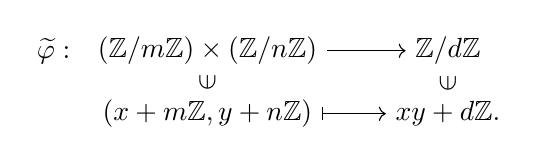
\begin{tikzpicture}[node distance=1mm]
  \node (functionName) at (0, 0) {$\widetilde{\varphi}:$};
  \node[right = of functionName] (domain)
    {$(\mathbb{Z}/m\mathbb{Z}) \times (\mathbb{Z}/n\mathbb{Z})$};
  \node[below = 2mm of domain] (element) {$(x + m\mathbb{Z}, y + n\mathbb{Z})$};
  \path (element)--(domain)node[midway,sloped] {$\in$};
  \node[right = 1cm of domain] (codomain) {$\mathbb{Z}/d\mathbb{Z}$};
  \node at (element-|codomain) (image) {$xy + d\mathbb{Z}.$};
  \path (image)--(codomain)node[midway,sloped] {$\in$};
  \draw[->] (domain) -- (codomain);
  \draw[|->] (element) -- (image);
\end{tikzpicture}
\end{center}
$\widetilde{\varphi}$ is well-defined and $\mathbb{Z}$-bilinear.
\item[(2)]
By the universal property,
$\widetilde{\varphi}$ factors through a $\mathbb{Z}$-bilinear map
$$\varphi: (\mathbb{Z}/m\mathbb{Z}) \otimes_{\mathbb{Z}} (\mathbb{Z}/n\mathbb{Z})
\to \mathbb{Z}/d\mathbb{Z}$$
(such that $\varphi(x \otimes y) = \widetilde{\varphi}(x, y)$).
\item[(3)]
To show that $\varphi$ is isomorphic, might find the inverse map
$\psi: \mathbb{Z}/d\mathbb{Z}
\to
(\mathbb{Z}/m\mathbb{Z}) \otimes_{\mathbb{Z}} (\mathbb{Z}/n\mathbb{Z})$
of $\varphi$.
Define $\psi$ by
\begin{center}
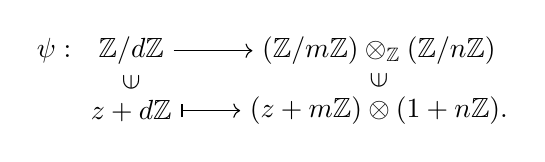
\begin{tikzpicture}[node distance=1mm]
  \node (functionName) at (0, 0) {$\psi:$};
  \node[right = of functionName] (domain) {$\mathbb{Z}/d\mathbb{Z}$};
  \node[below = 2mm of domain] (element) {$z + d\mathbb{Z}$};
  \path (element)--(domain)node[midway,sloped] {$\in$};
  \node[right = 1cm of domain] (codomain)
    {$(\mathbb{Z}/m\mathbb{Z}) \otimes_{\mathbb{Z}} (\mathbb{Z}/n\mathbb{Z})$};
  \node at (element-|codomain) (image) {$(z + m\mathbb{Z}) \otimes (1 + n\mathbb{Z}).$};
  \path (image)--(codomain)node[midway,sloped] {$\in$};
  \draw[->] (domain) -- (codomain);
  \draw[|->] (element) -- (image);
\end{tikzpicture}
\end{center}
$\psi$ is well-defined and $\mathbb{Z}$-linear.
\item[(4)]
$\psi \circ \varphi = \text{id}$.
\item[(5)]
$\varphi \circ \psi = \text{id}$. \\
\end{enumerate}



\emph{Proof of (1).}
\begin{enumerate}
\item[(a)]
\emph{$\widetilde{\varphi}$ is well-defined.}
Say $x' = x + am$ for some $a \in \mathbb{Z}$
and $y' = y + bn$ for some $b \in \mathbb{Z}$.
Then $x'y' - xy = yam + xbn + abmn \in \mathbb{Z}/d\mathbb{Z}$.
That is, $\widetilde{\varphi}$
is independent of coset representative.
\item[(b)]
\emph{$\widetilde{\varphi}$ is $\mathbb{Z}$-bilinear.}
\begin{enumerate}
\item[(i)]
\emph{For any $\lambda \in \mathbb{Z}$,
$\widetilde{\varphi}(\lambda x, y)
= \widetilde{\varphi}(x, \lambda y)
= \lambda \widetilde{\varphi}(x, y)$.}
In fact,
\begin{align*}
  \widetilde{\varphi}(\lambda(x+m\mathbb{Z}), y+n\mathbb{Z})
  &= \widetilde{\varphi}(\lambda x+m\mathbb{Z}, y+n\mathbb{Z})
  = \lambda x y + d\mathbb{Z}, \\
  \widetilde{\varphi}(x+m\mathbb{Z}, \lambda(y+n\mathbb{Z}))
  &= \widetilde{\varphi}(x+m\mathbb{Z}, \lambda y+n\mathbb{Z})
  = \lambda x y + d\mathbb{Z}, \\
  \widetilde{\varphi}(x_1+m\mathbb{Z}, y+n\mathbb{Z})
  &= \lambda (x y + d\mathbb{Z})
  = \lambda x y + d\mathbb{Z}.
\end{align*}
\item[(ii)]
\emph{$\widetilde{\varphi}(x_1 + x_2, y)
= \widetilde{\varphi}(x_1, y) + \widetilde{\varphi}(x_2, y)$.}
In fact,
\begin{align*}
  \widetilde{\varphi}((x_1+x_2)+m\mathbb{Z}, y+n\mathbb{Z})
  &= (x_1 + x_2) y + d\mathbb{Z}, \\
  \widetilde{\varphi}(x_1+m\mathbb{Z}, y+n\mathbb{Z})
  + \widetilde{\varphi}(x_2+m\mathbb{Z}, y+n\mathbb{Z})
  &= (x_1 y + d\mathbb{Z}) + (x_2 y + d\mathbb{Z}) \\
  &= (x_1 + x_2) y + d\mathbb{Z}.
\end{align*}
\item[(iii)]
\emph{$\widetilde{\varphi}(x, y_1 + y_2)
= \widetilde{\varphi}(x, y_1) + \widetilde{\varphi}(x, y_2)$.}
Similar to (ii).
\end{enumerate}
\end{enumerate}
$\Box$ \\



\emph{Proof of (3).}
\begin{enumerate}
\item[(a)]
\emph{$\psi$ is well-defined.}
Say $z' = z + cd$ for some $c \in \mathbb{Z}$.
Note that $d = \alpha m + \beta n$ for some $\alpha, \beta \in \mathbb{Z}$.
Thus
\begin{align*}
  \psi(z' + d\mathbb{Z})
  &= \psi(z + cd + d\mathbb{Z}) \\
  &= \psi(z + c(\alpha m + \beta n) + d\mathbb{Z}) \\
  &= (z + c(\alpha m + \beta n) + m\mathbb{Z}) \otimes (1 + n\mathbb{Z}) \\
  &= (z + c \beta n + m\mathbb{Z}) \otimes (1 + n\mathbb{Z}) \\
  &= (z + m\mathbb{Z}) \otimes (1 + n\mathbb{Z})
  + (c \beta n + m\mathbb{Z}) \otimes (1 + n\mathbb{Z}) \\
  &= \psi(z + d\mathbb{Z})
  + (1 + m\mathbb{Z}) \otimes (c \beta n + n\mathbb{Z}) \\
  &= \psi(z + d\mathbb{Z}).
\end{align*}
\item[(b)]
\emph{$\psi$ is $\mathbb{Z}$-linear.}
\begin{enumerate}
\item[(i)]
\emph{For any $\lambda \in \mathbb{Z}$,
$\psi(\lambda z) = \lambda \psi(z)$.}
In fact,
\begin{align*}
  \psi(\lambda(z + d\mathbb{Z}))
  &= \psi(\lambda z + d\mathbb{Z})
  = (\lambda z + m\mathbb{Z}) \otimes (1 + n\mathbb{Z}), \\
  \lambda \psi(z + d\mathbb{Z})
  &= \lambda((z + m\mathbb{Z}) \otimes (1 + n\mathbb{Z}))
  = (\lambda z + m\mathbb{Z}) \otimes (1 + n\mathbb{Z}).
\end{align*}
\item[(ii)]
\emph{$\psi(z_1 + z_2) = \psi(z_1) + \psi(z_2)$.}
\begin{align*}
  \psi((z_1 + z_2) + d\mathbb{Z})
  &= (z_1 + z_2 + m\mathbb{Z}) \otimes (1 + n\mathbb{Z}), \\
  \psi(z_1 + d\mathbb{Z}) + \psi(z_2 + d\mathbb{Z})
  &= (z_1 + m\mathbb{Z}) \otimes (1 + n\mathbb{Z})
  + (z_2 + m\mathbb{Z}) \otimes (1 + n\mathbb{Z}) \\
  &= (z_1 + z_2 + m\mathbb{Z}) \otimes (1 + n\mathbb{Z}).
\end{align*}
\end{enumerate}
\end{enumerate}
$\Box$ \\



\emph{Proof of (4).}
For any $(x + m\mathbb{Z}) \otimes (y + n\mathbb{Z}) \in
(\mathbb{Z}/m\mathbb{Z}) \otimes_{\mathbb{Z}} (\mathbb{Z}/n\mathbb{Z})$,
\begin{align*}
  \psi(\varphi((x + m\mathbb{Z}) \otimes (y + n\mathbb{Z})))
  &= \psi(xy + d\mathbb{Z}) \\
  &= (xy + m\mathbb{Z}) \otimes (1 + n\mathbb{Z}) \\
  &= (x + m\mathbb{Z}) \otimes (y + n\mathbb{Z}).
\end{align*}
$\Box$ \\



\emph{Proof of (5).}
For any $z + d\mathbb{Z} \in \mathbb{Z}/d\mathbb{Z}$,
\begin{align*}
  \varphi(\psi(z + d\mathbb{Z})
  &= \varphi((z + m\mathbb{Z}) \otimes (1 + n\mathbb{Z})) \\
  &= z + d\mathbb{Z}.
\end{align*}
$\Box$ \\\\



%%%%%%%%%%%%%%%%%%%%%%%%%%%%%%%%%%%%%%%%%%%%%%%%%%%%%%%%%%%%%%%%%%%%%%%%%%%%%%%%



\subsubsection*{Exercise 2.2.}
\addcontentsline{toc}{subsubsection}{Exercise 2.2.}
\emph{Let $A$ be a ring, $\mathfrak{a}$ an ideal, $M$ an $A$-module.
Show that $(A/\mathfrak{a}) \otimes_A M$ is isomorphic to $M/\mathfrak{a}M$.
(Hint: Tensor the exact sequence
$0
\rightarrow \mathfrak{a}
\rightarrow A
\rightarrow A/\mathfrak{a}
\rightarrow 0$ with $M$.} \\



\emph{Proof (Hint).}
There is a natural exact sequence $E$:
\[
  E: 0
  \rightarrow \mathfrak{a}
  \xrightarrow{i} A
  \xrightarrow{\pi} A/\mathfrak{a}
  \rightarrow 0
\]
where $i$ is the inclusion map (and $\pi$ is the projection map).
Tensor $E$ with $M$:
$$E':
\mathfrak{a} \otimes_{A} M
\xrightarrow{i \otimes 1} A \otimes_{A} M
\xrightarrow{\pi \otimes 1} (A/\mathfrak{a}) \otimes_{A} M
\rightarrow 0$$
is exact, or
$$(A/\mathfrak{a}) \otimes_{A} M \cong A \otimes_{A} M/\text{im}(i \otimes 1).$$
By Proposition 2.14,
There is an unique isomorphism $A \otimes_{A} M \to M$ defined by
$a \otimes x \mapsto ax$.
This isomorphism sends $\text{im}(i \otimes 1)$ to $\mathfrak{a}M$.
Therefore,
$$
(A/\mathfrak{a}) \otimes_{A} M \cong M/\mathfrak{a}M.$$
$\Box$ \\



\emph{Proof (Brute-force).}
\begin{enumerate}
\item[(1)]
Define $\widetilde{\varphi}$ by
\begin{center}
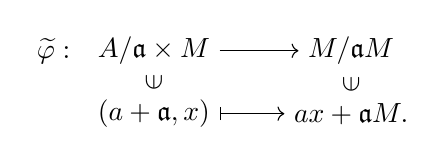
\begin{tikzpicture}[node distance=1mm]
  \node (functionName) at (0, 0) {$\widetilde{\varphi}:$};
  \node[right = of functionName] (domain)
    {$A/\mathfrak{a} \times M$};
  \node[below = 2mm of domain] (element) {$(a + \mathfrak{a}, x)$};
  \path (element)--(domain)node[midway,sloped] {$\in$};
  \node[right = 1cm of domain] (codomain) {$M/\mathfrak{a}M$};
  \node at (element-|codomain) (image) {$ax + \mathfrak{a}M.$};
  \path (image)--(codomain)node[midway,sloped] {$\in$};
  \draw[->] (domain) -- (codomain);
  \draw[|->] (element) -- (image);
\end{tikzpicture}
\end{center}
$\widetilde{\varphi}$ is well-defined and $A$-bilinear.
\item[(2)]
By the universal property,
$\widetilde{\varphi}$ factors through a $A$-bilinear map
$$\varphi: A/\mathfrak{a} \otimes_{A} M
\to M/\mathfrak{a}M$$
(such that $\varphi(a \otimes x) = \widetilde{\varphi}(a, x)$).
\item[(3)]
To show that $\varphi$ is isomorphic, might find the inverse map
$\psi: M/\mathfrak{a}M
\to
A/\mathfrak{a} \otimes_{A} M$
of $\varphi$.
Define $\psi$ by
\begin{center}
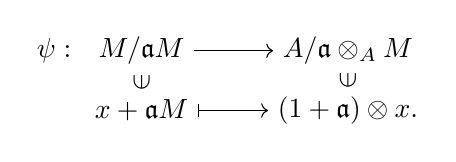
\begin{tikzpicture}[node distance=1mm]
  \node (functionName) at (0, 0) {$\psi:$};
  \node[right = of functionName] (domain) {$M/\mathfrak{a}M$};
  \node[below = 2mm of domain] (element) {$x + \mathfrak{a}M$};
  \path (element)--(domain)node[midway,sloped] {$\in$};
  \node[right = 1cm of domain] (codomain)
    {$A/\mathfrak{a} \otimes_{A} M$};
  \node at (element-|codomain) (image) {$(1 + \mathfrak{a}) \otimes x.$};
  \path (image)--(codomain)node[midway,sloped] {$\in$};
  \draw[->] (domain) -- (codomain);
  \draw[|->] (element) -- (image);
\end{tikzpicture}
\end{center}
$\psi$ is well-defined and $A$-linear.
\item[(4)]
$\psi \circ \varphi = \text{id}$.
\item[(5)]
$\varphi \circ \psi = \text{id}$.
\end{enumerate}
$\Box$ \\\\



%%%%%%%%%%%%%%%%%%%%%%%%%%%%%%%%%%%%%%%%%%%%%%%%%%%%%%%%%%%%%%%%%%%%%%%%%%%%%%%%



\subsubsection*{Exercise 2.3.}
\addcontentsline{toc}{subsubsection}{Exercise 2.3.}
\emph{Let $A$ be a local ring, $M$ and $N$ finitely generated $A$-modules.
Prove that if $M \otimes_{A} N = 0$, then $M = 0$ or $N = 0$.
(Hint: Let $\mathfrak{m}$ be the maximal ideal,
$k = A/\mathfrak{m}$ the residue field.
Let $M_k = k \otimes_{A} M \cong M/\mathfrak{m}M$ by Exercise 2.2.
By Nakayama's lemma, $M_k = 0 \Longrightarrow M = 0$.
But
$M \otimes_{A} N = 0
\Longrightarrow
(M \otimes_{A} N)_k = 0
\Longrightarrow
M_k \otimes_k N_k = 0
\Longrightarrow
M_k = 0 \text{ or } N_k = 0$
since $M_k$, $N_k$ are vector spaces over a field.)} \\

The conclusion might be false if $A$ is not local. For example, Exercise 2.1. \\



\emph{Proof (Hint).}
Let $\mathfrak{m}$ be the maximal ideal,
$k = A/\mathfrak{m}$ the residue field.
Let $M_k = k \otimes_{A} M$.
\begin{enumerate}
\item[(1)]
\emph{(Base extension) Show that
$(M \otimes_{A} N)_k = M_k \otimes_{k} N_k$.}
In fact, by Proposition 2.14
\begin{align*}
(M \otimes_{A} N)_k
&= k \otimes_{A} (M \otimes_{A} N) \\
&= (k \otimes_{A} M) \otimes_{A} N \\
&= M_k \otimes_{A} N \\
&= (M_k \otimes_{k} k) \otimes_{A} N \\
&= M_k \otimes_{k} (k \otimes_{A} N) \\
&= M_k \otimes_{k} N_k.
\end{align*}
\item[(2)]
\begin{align*}
M \otimes_{A} N = 0
&\Longrightarrow
(M \otimes_{A} N)_k = 0 \\
&\Longrightarrow
M_k \otimes_k N_k = 0
  &\text{((1))} \\
&\Longrightarrow
M_k = 0 \text{ or } N_k = 0
  &\text{($M_k, N_k$: vector spaces)} \\
&\Longrightarrow
M/\mathfrak{m}M = 0 \text{ or } M/\mathfrak{m}M = 0
  &\text{(Exercise 2.2)} \\
&\Longrightarrow
M = 0 \text{ or } N = 0.
  &\text{(Nakayama's lemma)} \\
\end{align*}
\end{enumerate}
$\Box$ \\\\



%%%%%%%%%%%%%%%%%%%%%%%%%%%%%%%%%%%%%%%%%%%%%%%%%%%%%%%%%%%%%%%%%%%%%%%%%%%%%%%%



\subsubsection*{Exercise 2.4.}
\addcontentsline{toc}{subsubsection}{Exercise 2.4.}
\emph{Let $M_i$ $(i \in I)$ be any family of $A$-modules,
and let $M$ be their direct sum.
Prove that $M$ is flat $\Leftrightarrow$ each $M_i$ is flat.} \\



\emph{Proof.}
Given any $A$-module homomorphism $f: N' \to N$.
\begin{enumerate}
\item[(1)]
Similar to Proposition 2.14(iii), we have
two isomorphisms
  \begin{enumerate}
  \item[(a)]
  $$\varphi:
  \bigoplus_{i \in I} (N' \otimes M_i)
  \cong
  N' \otimes_A \bigoplus_{i \in I} M_i$$
  defined by
  $$\varphi((x \otimes m_i)_{i \in I}) = x \otimes (m_i)_{i \in I}$$
  where $x \in N'$, $m_i \in M_i$ $(i \in I)$.
  \item[(b)]
  $$\psi:
  N \otimes_A \bigoplus_{i \in I} M_i
  \cong
  \bigoplus_{i \in I} (N \otimes M_i)$$
  defined by
  $$\psi(y \otimes (m_i)_{i \in I}) = (y \otimes m_i)_{i \in I}$$
  where $y \in N$, $m_i \in M_i$ $(i \in I)$.
  \end{enumerate}
\item[(2)]
$f: N' \to N$ induces an $A$-module homomorphism
$$f \otimes \text{id}_{M}: N' \otimes_A M \to N \otimes_A M.$$
\item[(3)]
$\psi \circ f \otimes \text{id}_{M} \circ \varphi$ defines an $A$-module homomorphism
$$\psi \circ f \otimes \text{id}_{M} \circ \varphi:
\bigoplus_{i \in I} (N' \otimes M_i) \to \bigoplus_{i \in I} (N \otimes M_i)$$
which sends $(x \otimes m_i)_{i \in I}$ to $(f(x) \otimes m_i)_{i \in I}$.
That is,
$$\psi \circ f \otimes \text{id}_{M} \circ \varphi
= \bigoplus_{i \in I} f \otimes \text{id}_{M_i}$$.
\item[(4)]
\emph{Show that $M$ is flat if and only if each $M_i$ is flat.}
Suppose $f$ is injective.
\begin{align*}
&\text{$M_i$ is flat $\forall \: i \in I$} \\
\Longleftrightarrow&
\text{$f \otimes \text{id}_{M_i}$ is injective $\forall \: i \in I$} \\
\Longleftrightarrow&
\text{$\bigoplus_{i \in I} f \otimes \text{id}_{M_i}$ is injective}
  &\text{(Injectivity)} \\
\Longleftrightarrow&
\text{$\psi \circ f \otimes \text{id}_{M} \circ \varphi$ is injective}
  &\text{((3))} \\
\Longleftrightarrow&
\text{$f \otimes \text{id}_{M}$ is injective}
  &\text{($\varphi$, $\psi$ are isomorphic)} \\
\Longleftrightarrow&
\text{$M$ is flat.}
\end{align*}
\end{enumerate}
$\Box$ \\\\



%%%%%%%%%%%%%%%%%%%%%%%%%%%%%%%%%%%%%%%%%%%%%%%%%%%%%%%%%%%%%%%%%%%%%%%%%%%%%%%%



\subsubsection*{Exercise 2.5.}
\addcontentsline{toc}{subsubsection}{Exercise 2.5.}
\emph{Let $A[x]$ be the ring of polynomials in one indeterminate over a ring $A$.
Prove that $A[x]$ is a flat $A$-algebra. (Hint: Use Exercise 2.4.)} \\

\emph{Proof (Hint).}
\begin{enumerate}
\item[(1)]
$A$ is a flat $A$-module by Proposition 2.14(iv).
\item[(2)]
As an $A$-module,
$$A[x]
\cong \bigoplus_{n \in \mathbb{Z}^+} Ax^n
\cong \bigoplus_{n \in \mathbb{Z}^+} A$$
(since $Ax^n \cong A$).
\item[(3)]
By Exercise 2.4, $A[x] \cong \bigoplus_{n \in \mathbb{Z}^+} A$ is flat.
\end{enumerate}
$\Box$ \\\\



%%%%%%%%%%%%%%%%%%%%%%%%%%%%%%%%%%%%%%%%%%%%%%%%%%%%%%%%%%%%%%%%%%%%%%%%%%%%%%%%



\subsubsection*{Exercise 2.8.}
\addcontentsline{toc}{subsubsection}{Exercise 2.8.}
\begin{enumerate}
\item[(i)]
  \emph{If $M$ and $N$ are flat $A$-modules, then so is $M \otimes_{A} N$. }

\item[(ii)]
  \emph{If $B$ is a flat $A$-algebra and $N$ is a flat $B$-module,
  then $N$ is flat as $A$-module.} \\
\end{enumerate}



\emph{Proof of (i).}
Given any exact sequence of $A$-modules
$0 \to N_1 \to N_2 \to N_3 \to 0$.
Since $M$ is flat,
\[
  0 \to N_1 \otimes_{A} M \to N_2 \otimes_{A} M \to N_3 \otimes_{A} M \to 0
\]
is exact.
Since $N$ is flat,
\[
  0 \to (N_1 \otimes_{A} M) \otimes_{A} N
  \to (N_2 \otimes_{A} M) \otimes_{A} N
  \to (N_3 \otimes_{A} M) \otimes_{A} N \to 0
\]
is exact.
By Proposition 2.14 (ii),
\[
  0 \to N_1 \otimes_{A} (M \otimes_{A} N)
  \to N_2 \otimes_{A} (M \otimes_{A} N)
  \to N_3 \otimes_{A} (M \otimes_{A} N) \to 0
\]
is exact, or $M \otimes_{A} N$ is flat.
$\Box$ \\



\emph{Proof of (ii).}
Given any exact sequence of $A$-modules
$0 \to N_1 \to N_2 \to N_3 \to 0$.
Since $B$ is a flat $A$-algebra ($A$-module),
$$0 \to N_1 \otimes_{A} B \to N_2 \otimes_{A} B \to N_3 \otimes_{A} B \to 0$$
is exact.
Since $N$ is a flat $B$-module,
$$0 \to (N_1 \otimes_{A} B) \otimes_{B} N
\to (N_2 \otimes_{A} B) \otimes_{B} N
\to (N_3 \otimes_{A} B) \otimes_{B} N \to 0$$
is exact.
By ``Exercise 2.15'' on page 27,
$$0 \to N_1 \otimes_{A} (B \otimes_{B} N)
\to N_2 \otimes_{A} (B \otimes_{B} N)
\to N_3 \otimes_{A} (B \otimes_{B} N) \to 0$$
is exact.
By Proposition 2.14 (iv),
$$0 \to N_1 \otimes_{A} N
\to N_2 \otimes_{A} N
\to N_3 \otimes_{A} N \to 0$$
is exact,
or $N$ is flat.
$\Box$ \\\\



%%%%%%%%%%%%%%%%%%%%%%%%%%%%%%%%%%%%%%%%%%%%%%%%%%%%%%%%%%%%%%%%%%%%%%%%%%%%%%%%



\subsubsection*{Exercise 2.9.}
\addcontentsline{toc}{subsubsection}{Exercise 2.9.}
\emph{Let $0 \to M' \to M \to M'' \to 0$ be an exact sequence of $A$-modules.
If $M'$ and $M''$ are finitely generated, then so is $M$.} \\



\emph{Proof.}
\begin{enumerate}
\item[(1)]
  Write
  \[
    0 \to M' \xrightarrow{f} M \xrightarrow{g} M'' \to 0.
  \]
  Also write
  \begin{align*}
    &x_1, \ldots, x_n \text{ as generators of } M', \\
    &z_1, \ldots, z_m \text{ as generators of } M''
  \end{align*}
  (since $M'$ and $M''$ are finitely generated).

\item[(2)]
  Since the map $g: M \to M''$ is surjective,
  there exists $y_j \in M$ such that $g(y_j) = z_j$ for $j = 1, \ldots, m$.

\item[(3)]
  \emph{Show that $M$ is generated by}
  \[
    f(x_1), \ldots, f(x_n), y_1, \ldots, y_m.
  \]
  Given any $y \in M$.
  \begin{align*}
    y \in M
    &\Longrightarrow g(y) \in M'' \\
    &\Longrightarrow g(y) = \sum_{j=1}^{m} s_j z_j \text{ where } s_j \in A \\
    &\Longrightarrow g(y) = \sum_{j=1}^{m} s_j g(y_j) \\
    &\Longrightarrow g(y) = g\left( \sum_{j=1}^{m} s_j y_j \right) \\
    &\Longrightarrow y - \sum_{j=1}^{m} s_j y_j \in \ker(g) = \text{im}(f) \\
    &\Longrightarrow \exists \: x \in M' \text{ such that } f(x) = y - \sum_{j=1}^{m} s_j y_j
  \end{align*}
  Write $x = \sum_{i=1}^{n} r_i x_i$ where $r_i \in A$.
  So,
  \begin{align*}
    y \in M
    &\Longrightarrow f\left( \sum_{i=1}^{n} r_i x_i \right) = y - \sum_{j=1}^{m} s_j y_j \\
    &\Longrightarrow \sum_{i=1}^{n} r_i f(x_i) = y - \sum_{j=1}^{m} s_j y_j \\
    &\Longrightarrow y = \sum_{i=1}^{n} r_i f(x_i) + \sum_{j=1}^{m} s_j y_j.
  \end{align*}
  Hence, every $y \in M$ is a linear combination of
  $f(x_1), \ldots, f(x_n), y_1, \ldots, y_m$,
  or $M$ is finitely generated
  (by $f(x_1), \ldots, f(x_n), y_1, \ldots, y_m$).
\end{enumerate}
$\Box$ \\\\



%%%%%%%%%%%%%%%%%%%%%%%%%%%%%%%%%%%%%%%%%%%%%%%%%%%%%%%%%%%%%%%%%%%%%%%%%%%%%%%%
%%%%%%%%%%%%%%%%%%%%%%%%%%%%%%%%%%%%%%%%%%%%%%%%%%%%%%%%%%%%%%%%%%%%%%%%%%%%%%%%



\end{document}